%%%%%%%%%%%%%%%%%%%%%%%%%%%%%%%%%%%%%%%%%%%%%%%%%%%%%%%%%%%%%%%%%%%%%%%%%%%
% * <sonya.hanson@choderalab.org> 2015-04-23T18:56:00.248Z:
%
% 
%
% HEADER: DON'T EDIT THIS!
%%%%%%%%%%%%%%%%%%%%%%%%%%%%%%%%%%%%%%%%%%%%%%%%%%%%%%%%%%%%%%%%%%%%%%%%%%%
% ^ <sonya.hanson@choderalab.org> 2015-04-23T18:57:46.938Z.
% But why not?

\documentclass[11pt]{article}

\title{ Advancing predictive physical modeling through focused development of model systems to drive new modeling innovations}

\usepackage[top=0.5in, bottom=0.5in, left=0.5in, right=0.5in]{geometry}
\usepackage{helvet}
\usepackage{url} % hypderref?
\usepackage{graphicx}
\graphicspath{{figures/}} % The figures are in a figures/ subdirectory.
\renewcommand{\familydefault}{\sfdefault}
\pagestyle{empty}
%\pagestyle{plain}

% Fancy page-width tables
\usepackage{tabularx}

% Use a package for framed boxes
\usepackage{mdframed}

\usepackage[T1]{fontenc}
\usepackage{amssymb}


\usepackage{setspace}
\usepackage{microtype}

\usepackage{amsfonts}
\usepackage{amsmath}

\usepackage{floatrow}

\usepackage[normalem]{ulem} % for nci.bst

\usepackage{sidecap}
\usepackage[abs]{overpic}
\usepackage{wrapfig}

%\usepackage[round,authoryear]{natbib}
\usepackage{cite}
%\setlength{\bibsep}{0.00in}

\usepackage{hyperref}
\hypersetup{colorlinks=true, urlcolor=black, citecolor=black, linkcolor=black}

\newcommand{\doi}[1]{\href{http://dx.doi.org/#1}{doi:#1}}

\newcommand{\ac}[1]{{\sc \lowercase{#1}}}

\renewcommand{\baselinestretch}{.93}
%\renewcommand{\baselinestretch}{.90}
\usepackage{wrapfig} 

\usepackage{bibspacing}
\setlength{\bibspacing}{\baselineskip}


\graphicspath{{figs/}}

\makeatletter

\newcommand{\captionfonts}{\footnotesize}

\makeatletter  % Allow the use of @ in command names
\long\def\@makecaption#1#2{%
  \vskip\abovecaptionskip
  \sbox\@tempboxa{{\captionfonts #1: #2}}%
  \ifdim \wd\@tempboxa >\hsize
    {\captionfonts #1. #2\par}
  \else
    \hbox to\hsize{\hfil\box\@tempboxa\hfil}%
  \fi
  \vskip\belowcaptionskip}      
\makeatother

\renewcommand{\figurename}{{\bf Figure}}

% Page numbering.
%\pagestyle{plain}
%\pagenumbering{arabic}

\setlength{\abovecaptionskip}{-5pt}

\makeatother

\renewcommand{\refname}{Bibliography and References Cited}

\setlength{\parindent}{0pt} % Don't indent first line
%\setlength{\parskip}{1ex plus 0.5ex minus 0.2ex} % Add some space between paragraphs
\setlength{\parskip}{0.8ex} % Add some space between paragraphs

\begin{document}

%======================================
% CITE OUR REFS FIRST
%\phantom{
%\cite{mobley-chodera-dill:2006:jcp:orientation-restraints,mobley-chodera-dill:2007:jctc:confine-and-release,shirts-mobley-chodera-pande:2007:jpcb:dispersion-corrections,chodera:jcp:2007,shirts-mobley-chodera:2007:annu-rep-comput-chem:prime-time,shirts-chodera:jcp:2008:mbar,ncmc,chodera-shirts:jcp:2011:gibbs,chodera:curr-opin-struct-biol:2011:drug-discovery,chodera-shirts:jcamd:2013:yank}
%\cite{gunner:biophys-j:1997:mcce,gunner:bba:2000:proton-electron-transfer,gunner:biophys-j:2002:mcce,gunner:j-comput-chem:2009:mcce2,gunner:jmb:2009:mcce2-hsa,gunner:proteins:2010:reaction-center,dutton:biochem:1994:photosynthetic-reaction-center,gunner:proteins:2010:reaction-center,gunner:photosynth-res:2013:photosynthetic-reaction-center,gunner:bba:2000:proton-electron-transfer,gunner:j-comput-chem:2009:mcce2,nielsen-gunner-garciamoreno:proteins:2011:pka-cooperative,stanton-houk:jctc:2008:benchmarking-pka-prediction}
%}

%%%%%%%%%%%%%%%%%%%%%%%%%%%%%%%%%%%%%%%%%%%%%%%%%%%%%%%%%%%%%%%%%%%%%%%%%%%
% SPECIFIC AIMS
%%%%%%%%%%%%%%%%%%%%%%%%%%%%%%%%%%%%%%%%%%%%%%%%%%%%%%%%%%%%%%%%%%%%%%%%%%%

%{\large \bf SPECIFIC AIMS}

%\eject

%%%%%%%%%%%%%%%%%%%%%%%%%%%%%%%%%%%%%%%%%%%%%%%%%%%%%%%%%%%%%%%%%%%%%%%%%%%
% SIGNIFICANCE
%%%%%%%%%%%%%%%%%%%%%%%%%%%%%%%%%%%%%%%%%%%%%%%%%%%%%%%%%%%%%%%%%%%%%%%%%%%


%NEED TO CAREFULLY CONSIDER GRAPHICS -- SOMETHING ON SIGNIFICANCE?

{\large \bf SIGNIFICANCE}
%2 pages

%Promise of physical methods, how they could transform drug discovery and the design of new small molecules for chemical biology
% (If space permits here we will allude also to how this could help with broader areas too such as engineering of biologics)
\textbf{Physical modeling is poised to transform drug discovery and chemical biology by enabling true molecular design.}
While modeling  is used extensively in drug discovery, its main role at present is to aid with idea generation or filter large libraries of compounds for screening. 
Instead, we imagine using computational techniques extensively to guide the design process. 
Consider a medicinal chemist in the not-too-distant future who has just finished synthesizing several new derivatives of an existing inhibitor, and has obtained binding affinity or potency data against the desired biomolecular target. 
Before leaving work, she generates ideas for perhaps 100 new compounds which could be synthesized next, setting her computer to work overnight. 
By morning, the idea compounds have been prioritized based on reliable predictions of their affinity for the desired target, selectivity against antitargets, solubility, and membrane permeability.  
{\color{red}[JDC: Should we say something about pharmacodynamics/kinetic and toxicity liabilities? We \emph{are} starting with HSA, after all.]}
The chemist looks through the predicted properties for the top few compounds, selecting some for synthesis. 
If synthesizing and testing each compound takes several days, this workflow compresses roughly a year's work into a few days.

While this workflow is not yet a reality, significant strides have been made in this direction on multiple fronts toward accurate, predictive physical models, binding affinities~\cite{mobley_perspective_2012, christ_accuracy_2014, deng_distinguishing_2015, sherborne_preprint_2016, schrodinger_accurate_2015, christ_binding_2016, cui_affinity_2016, verras_free_2016}, solubilities~\cite{Schnieders:2012:J.Chem.TheoryComput., park_absolute_2014, liu_using_2016}, selectivity and drug resistance~\cite{leonis_contribution_2013}, and membrane permeability~\cite{lee_permeability_2016, comer_permeability_2014}. 
A considerable amount of science and engineering still remains to make this vision a reality, but \textbf{given recent progress, the question now seems more one of \emph{when} rather than \emph{whether}.} 

Widespread availability of inexpensive graphics processing units (GPUs) have provided a 100-fold increase in price/performance over CPUs, while advances in automation~\cite{liu_lead_2013} and sampling protocols have helped simulation-based techniques reach the point where they now begin to be genuinely useful in guiding drug discovery for a limited \emph{domain of applicability}~\cite{mikulskis_large-scale_2014, homeyer_binding_2014, sherborne_preprint_2016,  schrodinger_accurate_2015, christ_binding_2016, cui_affinity_2016, verras_free_2016}.
Specifically, in some situations, free energy calculations appear to be capable of achieving RMS errors of 1-2 kcal/mol with current force fields, even in prospective applications, sufficient to drastically reduce the number of molecules that must be synthesized and assayed~\cite{shirts_free-energy_2010}.
As a consequence, pharmaceutical companies are beginning to use these methods in active discovery projects.

%Limitations of methods and of retrospective tests or application for methods improvements
\textbf{Despite progress, current physical modeling methodologies suffer from severe limitations hindering their widespread use in molecular design.}
For example, even ``small'' protein conformational conformational changes not gracefully handled by current methodologies can yield errors up to 5 kcal/mol in calculated binding free energies~\cite{lim_sensitivity_2016}, force field limitations still pose major challenges~\cite{rocklin_blind_2013}, and the inability to treat important chemical effects like protonation and tautomer equilibria drastically limits the domain of applicability.
{\bf For many pharmaceutically relevant systems, the most important sources of error---and modeling challenges---are not yet clear.}

Progress on addressing these challenges has been frustratingly slow, hindered by a lack of high-quality data and community focus.
{\bf Neither retrospective tests nor prospective application in active discovery projects provides the necessary impetus and data to rapidly overcome remaining barriers to widespread utility.}
Large-scale retrospective tests can assess \emph{retrospective} performance, but they do not provide accurate guidance on utility for prospective design, nor do they effectively identify the most important sources of error.
One issue with retrospective tests is that they can easily result in over-fitting, where researchers apply a variety of protocols until one achieves significant results by statistical chance~\cite{Nuzzo:2015:Nature}.
In retrospective tests, performance may also not be indicative of expected performance in applications because even well-meaning researchers can take advantage of prior knowledge. 
For example, if the binding mode of a ligand is already known crystallographically, a researcher may use that binding mode in retrospective tests, whereas prospective or design work would require first selecting among candidate binding modes, introducing substantial uncertainty unaccounted for in the retrospective statistics~\cite{mobley_predicting_2007, boyce_predicting_2009, mobley_perspective_2012}.
This also means that in retrospective tests, researchers almost invariably try far fewer methods than in prospective tests, resulting in much less new insight.
Prospective tests, in contrast, force researchers to anticipate a multitude of potential situations rather than only those observed in a known benchmark dataset.
Prospective application in actual discovery projects, while important, also does not provide the necessary impetus, partly because often, the predicted compounds are in fact never tested~\cite{christ_binding_2016} or the experimental data necessary to assess the quality of the predictions is absent---for example, because binding affinities are not measured or no crystallography is available. 

%Explain need for blind challenges and how D3R only fills part of need
{\bf To accelerate progress in quantitative predictive physical modeling, we need a series of community blind prediction challenges focused on pushing the limits of predictive techniques, beginning from problems which are just barely tractable with today's methods and advancing to problems just past the frontier.}
These challenges should be designed to have the necessary high quality experimental data, but also be prospective, predictive tests.
While the Drug Design Data Resource (D3R~\cite{gathiaka_d3r_2016}, discussed further below) provides an existing community blind challenge on protein-ligand binding, it focuses on using \emph{existing} pharmaceutical datasets, not on introducing new data in a carefully controlled manner in order to maximize community learning~\cite{gathiaka_d3r_2016}. 
D3R serves well to assess where we are now---but we need a carefully-designed effort focused on improving modeling.

%Discuss importance of SAMPL (including publication/citation count, previous successes in advancing the field, focus), need for funding to:
%   a. Continue SAMPL
%   b. Allow for "design" of SAMPL (rather than having it be driven by data availability)
%   b. Extend SAMPL to bridge to D3R rather than leaving a "capability gap" (here's where I explain why this is distinct from D3R -- this is crucial)
\textbf{Physical modeling accuracy advances most rapidly when progress toward a complex goal can be decomposed into separate tractable steps, as revealed by carefully collected and curated data.}
To make rapid progress, our field needs an effort which focuses on specific \emph{component} problems of the overall problem of interest, collects and curates data that highlights these problems, and drives progress via prospective challenges.
This process allows the entire community to learn from both methodological success and failure. 
The model we propose here has been proven to drive dramatic improvements in modeling, as evidenced by our {\bf Statistical Assessment of Modeling of Proteins and Ligands (SAMPL)} series of challenges. 
SAMPL, born out of frustration with the lack of venues for comparing predictive accuracy on a level playing field, was initiated by Anthony Nicholls of OpenEye software in 2007/2008~\cite{nicholls_predicting_2008}, and has run challenges approximately every two years since then~\cite{nicholls_samp1_2009, mobley_predictions_2009, geballe_sampl2_2010, geballe_sampl3_2012, mobley_blind_2014-1, muddana_sampl4_2014, bannan_blind_2016, yin_overview_2016}.
Governance transitioned to an unfunded academic collaboration during SAMPL3 in 2012; this collaboration ran subsequent challenges as SAMPL4 (2014) and SAMPL5 (2016).
The PI of this proposal (Mobley) was a primary organizer of SAMPL4/5 (2014--2016).
%SAMPL has always involved a component focused on calculation of solvation properties such as hydration free energies, but also introduced host-guest systems as model binding systems for SAMPL3--5 (2012--2016), supplementing protein-ligand challenges (on trypsin and HIV integrase) which appeared in SAMPL3-4 (2012--2014). 
Much as unit testing is an indispensible tool for discovering where bugs in a program are hiding when complex integration tests fail, exercises like SAMPL are valuable in pinpointing and correcting modeling errors when the overall performance fails to live up to expectations for complex pharmacological targets.
To accomplish this, SAMPL has historically focused on both simple challenges that attempt to isolate likely sources of modeling errors, such as physical properties of small molecules (hydration free energies, aqueous tautomer ratios, partition or distribution coefficients between aqueous and nonpolar phases) as well as small molecule binding to targets of reduced complexity (such as host-guest binding, trypsin-fragment binding, and small molecule screens against HIV integrase).
{\bf SAMPL has already been a tremendous resource for the community, resulting in roughly 100 publications (some are coming out as of this writing) which are typically cited 5--50 times or more each {\color{red} [full list of refs]}.}
%Add full list of references here.

Here, we \textbf{design a new series of SAMPL challenges specifically to maximize learning value to the community}.
Until now, this has been impossible, because SAMPL has been entirely unfunded; its very existence has required ``donation'' of data and time, giving us no ability to gather datasets tailored to our purpose. 
Our proposed new challenges bridge the gap between calculations of simple physical properties that isolate forcefield inaccuracies from sampling challenges, like hydration---which can already be calculated fairly accurately~\cite{mobley_blind_2014-1}---and the D3R Grand Challenges on protein-ligand binding, which are a major source of consternation for the community so far~\cite{ignjatovic_binding-affinity_2016, deng_large_2016, sunseri_d3r_2016, gathiaka_d3r_2016}.
Unless this gap is bridged, there is the very real possibility that modeling may simply continue to fall far short of expectations in pharmaceutical challenges like D3R for reasons which are unclear.
Here, we design challenges to highlight major reasons for failure and drive progress towards resolving them.


\textbf{Our major goal is to rapidly advance predictive modeling to where it can guide experimental work doing biomolecular design, and extension of the SAMPL challenges will do exactly that.} This work will play a vital role in enhancing the work being done on \emph{existing} data by D3R, helping prepare methods for application to the more challenging systems emerging from pharma in D3R's challenges. 

{\large \bf INNOVATION}
% 1 page

%SAMPL drives science in our groups and in the field
   %a. Give examples from our groups from prior SAMPLs
   %b. Examples from field in prior SAMPLs
Blind predictive challenges---and SAMPL in particular---have already led to important new science on method development, evaluation, robustness, and force field improvements. 
But they have not yet produced dramatic improvements in predictive molecular design, in part because \textbf{funding is necessary to design a systematic and progressive series of challenges motivating such improvements}. 
Previous SAMPL challenges have been valuable in isolation -- but failed to move the frontier because they were driven by data availability rather than purposeful design.
Here, we take the innovative step of designing SAMPL to advance physical modeling.

Several historical examples serve to highlight how SAMPL can foster innovation (though far more examples are available in our SAMPL bibliography below). 
The first several SAMPL challenges on hydration free energies had rather hit-and-miss performance, highlighting pitfalls of existing methods and force fields which led to marked improvements in PB models~\cite{nicholls_samp1_2009, ellingson_analysis_2010,ellingson_efficient_2014}, recognition of some limitations of fixed-charge force fields ~\cite{mobley_alchemical_2012, Fennell:2014:J.Phys.Chem.B},
repair of some of these force field deficiencies via additional polarization or introduction of off-site charges~\cite{mobley_alchemical_2012, Fennell:2014:J.Phys.Chem.B, paranahewage_predicting_2016},
and helped motivate alternate implicit or hybrid solvent models~\cite{sulea_predicting_2011, li_testing_2014, brini_adapting_2016}.
{\color{red}{Together these advances led to a marked improvement in accuracy for calculations of hydration free energies between SAMPLX and SAMPLY (Figure []).}}
%FILL IN DETAILS ON LINE ABOVE
%
%Add some sort of a figure on how SAMPL has helped community -- maybe compare accuracy in hydration free energies (simple?!?) in an early SAMPL with accuracy on log D in this SAMPL or something similar? Show something that demonstrates progress.
%b.1 Figure showing progression in hydration free energy accuracy across a couple of SAMPLs or comparing two SAMPLs?
%
 %Fennell SEA, etc.
Shifts in protonation state and tautomer proved particularly important in the recent SAMPL5 logD challenge~\cite{bannan_blind_2016, klamt_prediction_2016}.
This challenge provided a tractable opportunity to isolate and explore these specific physical effects, which are so important in protein-ligand binding, while avoiding the full complexity of pharmaceutical binding studies.
Host-guest binding studies have also been particularly important~\cite{mobley_predicting_2016},
highlighting the importance of salt effects~\cite{yin_overview_2016, muddana_blind_2014, mobley_predicting_2016}
and in some cases revealing more severe force field limitations than observed in hydration and distribution challenges~\cite{yin_sampl5_2016, muddana_sampl4_2014-1}, pointing the way forward for improving predictive models of molecular interactions~\cite{yin_toward_2015, mobley_predicting_2016}.



%c. Mention uniqueness of SAMPL -- there are other predictive challenges (D3R, pKa coop, CASP) but none focused on driving quantitatively predictive protein-ligand modeling
This work is also innovative because of the uniqueness of SAMPL.
While there are other predictive challenges in the area of biomolecular modeling, such as D3R~\cite{gathiaka_d3r_2016}, the pKa cooperative~\cite{Nielsen:2011:Proteins}, CAPRI~\cite{Janin:2005:ProteinScience} and CASP~\cite{Moult:2014:Proteins},
\textbf{no other effort focuses specifically on driving predictive quantitative protein-ligand modeling}.
The SAMPL expansion we propose here is unique in its \emph{specific design} to drive improvements in modeling accuracy rather than simply serving an evaluative role.
SAMPL benefits the whole modeling community---for example, protein-ligand docking software has improved as a direct result of SAMPL hydration challenges~\cite{coleman_sampl4_2014}, and commercial software vendors have introduced new features or scientific improvements based on participation in SAMPL challenges~\cite{reinisch_prediction_2012, klamt_prediction_2016}.
In effect, {\bf SAMPL serves as an engine to spur innovation by new soliciting novel approaches to complex problems from the community and evaluating their success at predictions.}
 

% Innovation in experimental pipelines (Aim 3)
This work also focuses on innovative experimental methods.
Specifically, in Aim 3, we develop a new informatics platform to facilitate the rapid identification and study of particularly informative protein-ligand systems that are both experimentally tractable for high-throughput biophysical measurements and focus on specific challenges of interest.
We employ a fully automated wetlab to screen potential model systems for expression, carry out high-accuracy biophysical measurements, and perform automated error analysis to carefully assess experimental uncertainty.
%The Chodera lab---responsible for Aim 3---has substantial expertise in the area of automation of biophysical measurements and uncertainty analysis~\cite{Hanson:2015:JournalofComputer-AidedMolecularDesign}. 
%Cutting -- expertise is established elsewhere and is not relevant to innovation.
\textbf{This work is at the forefront of innovation in high-throughput, automated biophysical experiments to produce high quality data with well-characterized uncertainties.} 
Not only will the data itself be of prime importance, but the techniques themselves will help future experiments.

% Innovative reference calculations (Aim 4)
In Aim 4, in addition to running SAMPL challenges, we will also perform reference calculations with the latest techniques, testing their accuracy to assess the current state-of-the-art.
Both the Mobley and Chodera labs are experts in development of free energy methods for application to physical properties (e.g., ~\cite{mobley_blind_2014-1, Beauchamp:2015:JournalofPhysicalChemistryB, bannan_calculating_2016} and binding (e.g.,~\cite{rocklin_blind_2013, lim_sensitivity_2016, wang_identifying_2013}), and \textbf{these reference calculations will drive innovation} as well, serving several key roles: (1) Benchmarking the latest method developments against current ``best practices'' methods (by doing calculations via both approaches); (2) Facilitating learning, allowing others to compare against our results to determine how a change in method or force field impacts results; (3) Focusing the field on key issues by doing sensitivity analysis to whether conditions such as ionic strength, protonation state, tautomer choice, etc., impact computed values.

Careful challenge analysis also facilitates innovation, as tracking down \emph{why} models are failing and what particular problems still need attention is an in important and powerful aspect of SAMPL.
Much of this is left to the participants, but as organizers we do a great deal of work spotting patterns and providing a venue for participants to explore these issues.
When methods differ in performance, it is critical to understand whether the differences are statistically significant and important, and to provide an accurate accounting of the uncertainty in performance measures. 
Thus, careful and innovative analysis of challenge outcomes is particularly important in SAMPL~\cite{mobley_blind_2014-1, bannan_blind_2016, yin_overview_2016}, in some cases driving experimentation with new performance metrics~\cite{mobley_blind_2014-1}.




{\large \bf APPROACH}
% 9 pages

Our approach to systematically advancing modeling for biomolecular design involves collecting carefully targeted experimental datasets for challenges focusing on physical property prediction, host-guest binding, and protein-ligand binding.
These isolate individual limitations in quantitative physical modeling to solicit and evaluate multiple solutions from the community.
Aims 1--3 focus on tailoring and generating this experimental data, while Aim 4 focuses on fielding annual SAMPL challenges.
Aims 1--3 bring together multiple laboratories and both theorists and experimentalists: graduate students from the Mobley and Chodera laboratories are paired with well-equipped experimental groups in industry to collect physical property data (Aim 1); Gibb and Isaacs, leading experimentalists in supramolecular chemistry, work with theorist Mobley to perform host-guest affinity measurements (Aim 2); and the Chodera lab applies new automated approaches to identify suitable protein-ligand systems and measure binding (Aim 3).
The annual SAMPL challenges organized by the Mobley and Chodera labs (Aim 4) will evaluate best-practices reference calculations, feature both biennial physical meetings (coordinated with D3R) and virtual communication platforms to maximize community engagement, develop novel statistical analyses to identify and respond to problem areas, release benchmark datasets alongside primary experimental data, organize special journal issues to report progress, and encourage tool automation whenever possible.
%For space reasons, could reduce the summary above dramatically?

{\bf \underline{Aim 1}: Collect new physical property datasets to assess accuracy and spur improvements in force fields and modeling of protonation states and tautomers.} 
%\subsection{blah}
%Note to self: It would really be nice to make the Aim headers be bigger. Can I do that?
%Chodera suggests possibly {\bf \large}, or underlining Aim 1. 

Simple physical properties such as solvation, partitioning, and protonation equilibria can be calculated quite precisely with physical methods, allowing quantitative comparison of calculated values with experimental measurements and revealing and isolating deficiencies in our current models. 
For example, these properties allow us to directly probe force field accuracy and chemical effects like protonation and tautomer handling in the absence of slow conformational changes and other affects which complicate assessment in protein-ligand systems. 

{\bf Rationale:}
%Compare log D accuracy vs hydration accuracy, highlight issues and explain relevance to drug discovery; note lessons learned in SAMPL5
     %Maybe use a figure on log D accuracy?
We will generate new solution-phase physical property measurements for drug-like molecules to motivate improvements in force fields and handling of protonation states and tautomers.
This builds on our work on water-cyclohexane distribution coefficients for SAMPL5, done in partnership with Genentech, which revealed major problems with handling of protonation states and tautomers~\cite{bannan_blind_2016}  as well as serious forcefield limitations~\cite{paranahewage_predicting_2016}.
Distribution coefficients serve well to assess the state of the art and drive innovation, as they relate to transfer free energies from aqueous high-dielectric to low-dielectric environments, capturing many of the characteristics of transfer of drugs from water into binding sites but absent challenges with receptor conformational sampling and specific ligand-receptor interactions.
In SAMPL5, distribution coefficients were challenging enough that many methods performed poorly, with even the best methods having accuracies less than would be expected based on hydration free energies in water~\cite{bannan_blind_2016}, yet failures were informative and the major sources of error were issues which will also plague prediction of ligand-receptor interactions.
In some respects, distribution coefficients posed the ideal SAMPL challenge, hitting the sweet spot in terms of difficulty---difficult enough that clear failures were frequent, with ample room for improvement, but not so difficult that the reasons for failure were unclear in general. 
Still, many models consistently disagreed with experiment for particular compounds~\cite{paranahewage_predicting_2016, klamt_prediction_2016, bannan_blind_2016, rustenburg_measuring_2016}, revealing the impact that targeted follow-up experiments (such as those we will conduct here) could have on improving models.
%Our choice of cyclohexane-water distribution coefficients rather than octanol-water was motivated by both complexities with octanol experiments (~\cite{bannan_calculating_2016}, making it difficult to ensure the system modeled is the same one simulated) and potential sampling problems in octanol~\cite{Kollman:1996:AccountsofChemicalResearch}, though challenges we propose here will broaden past cyclohexane.
%This seems out of place, is here mainly to answer a question about what we did in the past ("why didn't you use octanol?"), and doesn't strengthen our plan for the future. Given the tightness of space, I'm cutting this. Also, our discussion of introducing octanol, below, implies why it wasn't used previously.

%Talk about limitations of approach -- lack of ability to do follow up expeirments, get the dynamic range we wanted, test things again after SAMPL? 
% Sustained funding will allow us to do that. 
% (This will also help answer the argument that we don't need funding for this...)
\textbf{This new experimental data is critical to maximize impact on the modeling community.} 
While the community has already benefitted considerably from SAMPL, as indicated by the nearly 100 publications on SAMPL [refs], the citation count, and lessons learned, the benefits are not what they could have been if the effort had funding.
%Re-insert SAMPL references here
A funded, coordinated effort allows the targeted collection of datasets designed to focus on the most important problems. 
With multiple investigators and collaborators, we are poised to respond and adapt to new challenges and opportunities which emerge in a manner not previously possible.
Additionally, we will be able to continue experimental work until the necessary data is collected rather than terminating it at a specific time point dictated by industry funding -- allowing us to do things like ensure the full dynamic range of $\log D$ values is covered, unlike in SAMPL5~\cite{rustenburg_measuring_2016, bannan_blind_2016}.
This will improve our ability to learn from the data -- for example, the lack of dynamic range for SAMPL5 meant that, when calculated values often spanned a larger dynamic range than the experimental values, it was unclear if this was an artifact of the data set itself, experimental limitations, or force field problems~\cite{rustenburg_measuring_2016, bannan_blind_2016, paranahewage_predicting_2016, klamt_prediction_2016}. 
With funding to extend the experimental set via follow-up experiments, we will be able to resolve similar issues, providing further impetus to improve models.

Below, we summarize plans for SAMPL6-10, though we will adapt to new opportunities as they arise and respond to persistent difficulties by ensuring the challenge is repeated with new data until clear improvement is seen.

%Explain what science -- log D/logP, pKa primarily but mention possible other areas of interest
{\bf SAMPL6: Cyclohexane/water and octanol/water distribution coefficients.}
Building on the success of distribution coefficient measurements in SAMPL5 and their surprising ability to motivate rapid advances in physical modeling methodologies~\cite{bannan_blind_2016}, we will measure cyclohexane-water distribution coefficients at pH 7.4 for a new batch of commercially-available drug- and fragment-like molecules.
%{\color{red}[JDC: Maybe the set can be broken into classes of varying chemical complexities? In general, I think clever experimental design ideas---indications we have really thought through how to maximize value---will be rewarded by the reviewers.]}
%DLM: Need to revisit this comment.
Given the routine nature of octanol-water distribution coefficient measurements and indications that their prediction may be computationally tractable~\cite{Bhatnagar:2013:PhysicalChemistryChemicalPhysics, bannan_calculating_2016} despite the heterogeneous structure of the wet octanol phase~\cite{Kollman:1996:AccountsofChemicalResearch}, we will also measure octanol-water distribution coefficients for the same compounds.
Because pKa prediction was difficult but critical for SAMPL5, we will focus SAMPL6 on forcefields and tautomers by measuring pKa values, revisiting pKa prediction in SAMPL7 and 8.

{\bf SAMPL7: pKa measurements for drug-like molecules.} 
While much less complex than protein-ligand affinities, distribution coefficient measurements still conflate the challenging issues of protonation state and tautomer prediction, as well as transfer into different environments which may contain small but important quantities of cosolvents. 
Thus, we will separate these issues and improve our handling of them one at a time. 
For SAMPL7, then, we will measure pKa values for an extensive set of drug-like molecules in water which will serve as the focus of the challenge, paving the way for SAMPL8.

{\bf SAMPL8: pKa measurements and distribution coefficients.}
In the next challenge, we will re-combine the pKa and transfer issues, measuring distribution coefficients \emph{and} pKa values for the same set of compounds, with participants predicting (a) distribution; (b) pKa; and (c) partition. 
Unlike SAMPL6, pKa values will not be provided.

{\bf SAMPL9-10.}
We will focus on solubility prediction in SAMPL9, and membrane permeability in SAMPL10, because of new computational developments.
With solubility predictions now becoming tractable~\cite{Schnieders:2012:J.Chem.TheoryComput., park_absolute_2014, liu_using_2016} (with Schr\"{o}dinger also working on amorphous solubility prediction), solubility measurements will be a valuable test for SAMPL9, combining the solvation aspects of SAMPL1-8 with a new solid phase component.
New computational techniques are targeting membrane permeability~\cite{lee_permeability_2016, comer_permeability_2014}, and this is experimentally accessible (see support letters from Pfizer and Merck), leading to our interest in permeability for SAMPL10.
%Alternatively, partition/distribution into other environments aside from cyclohexane or octanol may provide significant value, especially given dielectric constant issues posed by current force fields [ref].
%cite something by Fennell here
  
 %Industry partnerships (and past precedent)
{\bf Experimental plan:}
Experimental data will be collected in collaboration with our pharma partners (see support lettters), roughly following the model used for SAMPL5, where Chodera lab student Bas Rustenburg went to to Genentech to conduct cyclohexane-water logD measurements by adapting a Genentech high-throughput mass spectrometry workflow~\cite{rustenburg_measuring_2016}.
To collect physical property measurement datasets for SAMPL6-10, the Mobley and Chodera labs will send graduate students on visits or internships to industry collaborators to collect targeted datasets.
Working with industry collaborators (see Letters of Collaboration from Genentech, Pfizer, and Merck) gives us substantial access to equipment and high-throughput measurement workflows---such as the Sirius T3 from Sirius Analytical (which can measure partition/distribution coefficients, p$K_a$s, and solubilities for molecules with titratable groups), automation equipment, and compound libraries---for the purposes of rapidly collecting targeted datasets.
% add GSK if their letter comes in
Our previous experience demonstrates this model will work~\cite{rustenburg_measuring_2016}, and our partners see the value of this data and the SAMPL challenge to the modeling community.

Overall, Aim 1 extends prior SAMPL challenges via data focused on quantitative prediction of physical properties of tremendous relevance to accurately predicting biomolecular interactions, paving the way to applications in more complex systems addressed in Aims 2 and 3.

%Aim 2 (2 pages)
\textbf{\underline{Aim 2}: Measure affinities of drug-like compounds in supramolecular hosts to challenge quantitative models of binding in systems lacking major receptor sampling issues.}

\begin{wraptable}{r}{6.5cm}
\footnotesize
\begin{tabular}{l | l}
{\bf drug} & {\bf features} \\
\hline
memantine & adamantane; 1:1 \\
saxagliptin & adamantane; 1:1 \\
premarin & steroid \\
pancuronium & steroid\\
varenicline & 1:1 vs 1:2 \\
valsartan & pKa 4.37 \\ 
omeprazole & pKa 4.77 \\
ranolazine & pKa 7.17; epitopes \\
pradaxa & pKa 3.87; epitopes \\
nilotinib & epitopes; pKa 6.3 \\
sensipar & epitopes; folding \\
vyvance & diamine; epitopes; folding \\
minocycline & tetracyclin; amino aniline \\
\end{tabular}
\caption{\label{table:CB} {\bf Selected drugs whose binding to CB[$n$] hosts will be assayed for SAMPL6, 8, and 10 challenges (SA 2.1).} These drugs bind to the cucubituril-based host systems considered here, some at high affinity, so measuring their affinities provides a way to test methods for predicting binding interactions absent complexities present in protein-ligand systems.
}
\end{wraptable}



%Intro lessons learned on HG systems, relevance to drug discovery
Aim 1 focuses on the behavior of small molecules and its environment-dependence, in the absence of receptors and the associated potential for slow sampling, strong specific interactions, and other challenges such as salt effects.
Binding in host-guest systems retains many of the same challenges seen in Aim 1 and introduces strong specific interactions and other challenges like salt effects~\cite{mobley_predicting_2016}, while still avoiding many of the issues with slow sampling (of protein conformational changes, ions, and ligand binding modes) seen in protein-ligand interactions.
Thus, new data for SAMPL challenges on host-guest binding is critical to provide challenges of intermediate complexity between those of physical properties and those in bioolecular binding---but binding in host-guest systems introdyin_overview_2016uces a wider variety of challenges relevant to biomolecular interactions, but without the full array of challenges seen in protein-ligand interactions, as reviewed recently
Thus, we believe that host-guest binding provides a critical step towards accurately modeling biomolecular interactions, focusing the field on issues not commonly encountered in physical property challenges (such as the importance of accurately modeling ionic conditions) that are highly relevant for protein-ligand interactions.
Already, over the past several SAMPL challenges, host-guest systems have provided key tests for modeling of binding interactions, resulting in new attention paid to how co-solvents and ions modulate binding (resulting in errors of up to 5 kcal/mol when these effects are neglected) and the importance of adequately sampling water rearrangements~\cite{muddana_sampl4_2014, mobley_predicting_2016, yin_overview_2016, bhakat_resolving_2016}. 
Host-guest binding proves remarkably difficult to model accurately~\cite{henriksen_computational_2015}, in part due to force field limitations (resulting in new force field work~\cite{yin_toward_2015}).
%{\color{red}[JDC: Assuming convergence is achieved, that leaves only forcefield limitations and protonation/tautomer effects. How can these contributions be dissected or separated, and how can is failure or success specifically able to drive progress?]}
%Dissected -- by measuring protonation for example, I suppose (but I don't think we can expand on that here...?) 
%How is failure or success able to drive progress -- it seems like I just said that; people start focusing on these issues and working to resolve them. DId you have something specific in mind?

Here, we design a series of SAMPL challenges focused on two classes of host-guest systems---cucurbiturils and derivatives (SA 2.1) and Gibb's deep-cavity cavitands (GDCCs, SA 2.2)---both of which build on prior SAMPL challenges.
These two sets of systems exhibit different challenges as recently reviewed~\cite{mobley_predicting_2016}, with the hosts of 2.1 bringing relatively modest co-solvent and ion effects but some receptor sampling problems for the acyclic hosts, and the GDCCs of 2.2 bringing profound ion and co-solvent effects as well as water sampling challenges.
Methods which perform well on one class may not perform well on the other~\cite{mobley_predicting_2016}, since the distinct sets of challenges highlight different limitations.
This diversity drive more innovation than would a focus on a single host class.

%Chodera suggested this on the octa-acid section:
%* We need to emphasize why the octa-acid system has proven to be so valuable for modelers in the introduction: What specific physical challenges does the system probe, and what have we learned? We also need to add citations to the meta-analysis and maybe even all of the papers that addressed this system. David can likely address this.
%DLM: It's tempting to add material along these lines to the beginning of both the octa-acid and CB sections (i.e. making each start with a "history" section), and I certainly have material on that, but given that we're a bit over a page too long before I even add figures, I'll leave this as a placeholder in case we somehow find ourselves with space to add it. We can't afford the space at present unless we find something to shrink dramatically.


{\bf Subaim 2.1: Cucurbituril-based receptors as model binding systems}
%Isaacs science

\textbf{Cucurbituril derivatives for host-guest binding.} 
%DLM: A bit odd to have the OA section start with a history header and this one not. May need to address.
Building on previous success with cucurbit[$n$]uril (abbreviated CB[$n$]) experiments for SAMPL challenges~\cite{ma_acyclic_2012-2, cao_absolute_2014, she_glycoluril-derived_2016}, we will conduct a series of new experiments on these receptors for five new challenges,
 with experimental work conducted by co-investigator Isaacs, an expert on these systems who provided data for previous SAMPL challenges.
CB[$n$] receptors are particularly well suited to our goals because they exhibit: (1) high binding affinities toward suitable guests in water comparable to protein-ligand affinities (routinely $\mu$M to nM; occasionally pM to fM)~\cite{cao_attomolar_2014, liu_cucurbituril_2005, mock_structure_1986, assaf_cucurbiturils:_2015, moghaddam_new_2011, shetty_can_2015, biedermann_release_2012}, (2) high selectivities between structurally related guests which translate into large $\Delta \Delta G$ values~\cite{isaacs_stimuli_2014}, (3) low molecular weights (1--2 kDa) permitting high levels of theory to be used, and (4) highly restricted conformational degrees of freedom, reducing conformational sampling challenges often seen in protein-ligand binding.
For SAMPL6-10, we will resynthesize a series of CB[$n$]-type receptors of increasing complexity, measure $K_a$ values, and determine host-guest stoichiometry and geometry toward pharmaceutically relevant guests (selected drugs) in order to stringently test methods for predicting binding.  
Figure~\ref{figure:CB} shows the chemical structures of three hosts---Me$_4$CB[8]~\cite{vinciguerra_synthesis_2015}, glycoluril hexamer~\cite{lucas_templated_2011}, and acyclic CB[$n$]-type receptors~\cite{ma_acyclic_2012, ma_acyclic_2012-1, zhang_acyclic_2014, gilberg_acyclic_2015, sigwalt_acyclic_2016, zhang_acyclic_2014-1} which span a range in terms of level of preorganization and formal charge.

\begin{figure}[h]
\begin{centering}
\resizebox{\textwidth}{!}{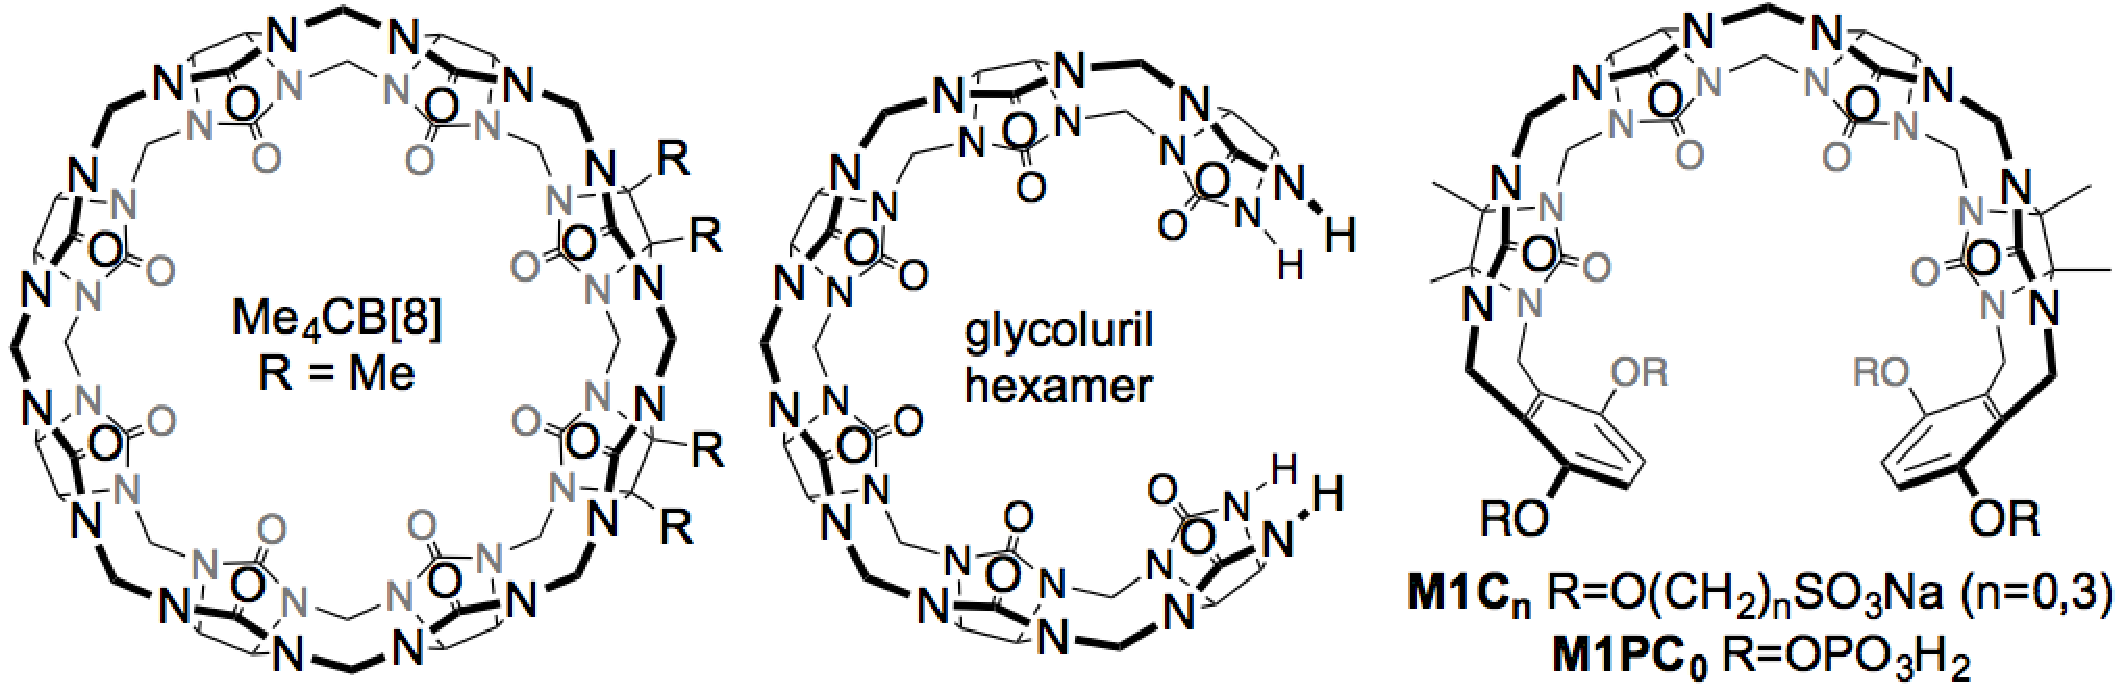
\includegraphics{figures/CB.pdf}}

\end{centering}

\vspace{0.1in}
\caption{\label{figure:CB} \footnotesize {\bf Structures of Me$_4$CB[8], glycouril hexamer, and acyclic CB[n]-type receptors.} These receptors bind a variety of drug-like molecules, some with high affinity, and this binding will form the basis of a cucubituril-based series of SAMPL binding challenges.}

\end{figure}

\textbf{SAMPL6-10 cucurbituril challenges.} 
\emph{For SAMPL6}, we will measure $K_a$ and $\Delta H$ values, stoichiometry, and geometry for the interaction of Me$_4$CB[8] (a soluble CB[8] derivative) with 15 guests (selected top drugs, Table~\ref{table:CB}) by either direct or competition isothermal titration calorimetry (ITC), UV/Vis or fluorescence indicator displacement assay, or NMR competition experiments, as previously~\cite{cao_attomolar_2014, liu_cucurbituril_2005, ma_acyclic_2010, she_glycoluril-derived_2016}.  
Our selection of Me$_4$CB[8] binding to top drugs allows us to modulate the computational complexity by: 1) changing host flexibility (e.g. Me$_4$CB[8] can exhibit ellipsoidal deformation)~\cite{vinciguerra_synthesis_2015}, 2) allowing the possibility of binary or ternary (e.g. 1:1 and/or 1:2 host:guest) complexes~\cite{ko_supramolecular_2007, barrow_cucurbituril-based_2015, urbach_molecular_2011}, 3) using drugs with several potential binding epitopes or modes to induce sampling issues.  Host:guest stoichiometry and geometry (e.g., which binding epitope is complexed) will be addressed by ITC $n$ values, Job plots monitored by UV/Vis or NMR~\cite{connors_binding_1987}, and by $^1$H NMR complexation induced changes in chemical shifts~\cite{masson_cucurbituril_2012}.  
All studies will be conducted in phosphate buffered saline (p$H$ 7.4 with physiological salt) which introduces its own complexities due to salt competition for binding~\cite{marquez_mechanism_2004, mobley_predicting_2016}. 
\emph{SAMPL7} will revisit the same host, but use 15 different guests be selected from commercial sources on the basis of reference calculations (on a larger set of guests) to ensure that they cover substantial dynamic range and/or exhibit affinities that depend substantially on the force field or water model, thus effectively testing our force fields and methods.
For \emph{SAMPL8}, we will focus on binding of the same 15 drugs (Table~\ref{table:CB}), but to glycoluril hexamer. 
This host introduces the complication of increased conformational dynamics, and influences the number and energy of solvating (and unusually coordinated) water molecules implicated in the high binding constants for CB[$n$]-guest complexes~\cite{biedermann_release_2012, biedermann_hydrophobic_2014}.  
The selected drugs include several with p$K_a$ values in the 3.8 to 7.4 range; given that CB[$n$]-type receptors (like biomolecular receptors) can induce pKa shifts in their guests of up to 4 pKa units~\cite{saleh_activation_2008, nau_deep_2011, ghosh_strategic_2012}, this will test how well models can predict these effects. 
Additionally, it will couple nicely with the focus on p$K_a$ values in Aim 1.
\emph{SAMPL9} will revisit glycouril hexamer with the same 15 guests from \emph{SAMPL7}.
\emph{SAMPL10} will shift to acyclic CB[$n$]-type receptors (e.g. M1C$_3$, M1C$_0$, and M1PC$_0$ that contain anionic solubilizing groups attached via different linker lengths.  
As in SAMPL3~\cite{muddana_sampl3_2012}, these acyclic CB[$n$]-type receptors introduce conformational complexity, and water interactions play a key role.
Moreover, the presence of 4 anionic groups near the cavity will likely impact balance between ion-dipole interactions and the solvation of the free host.

{\bf Subaim 2.2. Gibb deep cavity cavitands for host-guest studies} 

%Gibb science

{\bf History of octa-acid SAMPL challenges.} During SAMPL4~\cite{gibb_binding_2013} and SAMPL5~\cite{sullivan_binding_2016} we focused on two hosts: the octa-acid 1 (R = H) and another octa-acid derivative with four methyl groups positioned at the portal of the binding pocket (1, R = Me). 
These studies used isothermal titration calorimetry (ITC) to measure the thermodynamics of (1) host {\bf 1} (R = H) complexing a range of 9 carboxylate guests,
and (2) the binding of 6 carboxylate and trimethylammonium guests to both hosts ({\bf 1}, H = H and Me; Figure~\ref{figure:gdccs}).  
In both cases $^1$H-NMR titration was also used to confirm ITC-derived free energies of binding.  
As noted above, co-solvent effects and water rearrangements posed particular challenges for predicting binding in these hosts. 
SAMPL5 emphasized how differences in the shape of the hydrophobic pocket of the host can have a profound affect on affinity for some guests~\cite{yin_overview_2016}.
% Comment on value to community

\begin{figure}[h]
\begin{centering}
\resizebox{\textwidth}{!}{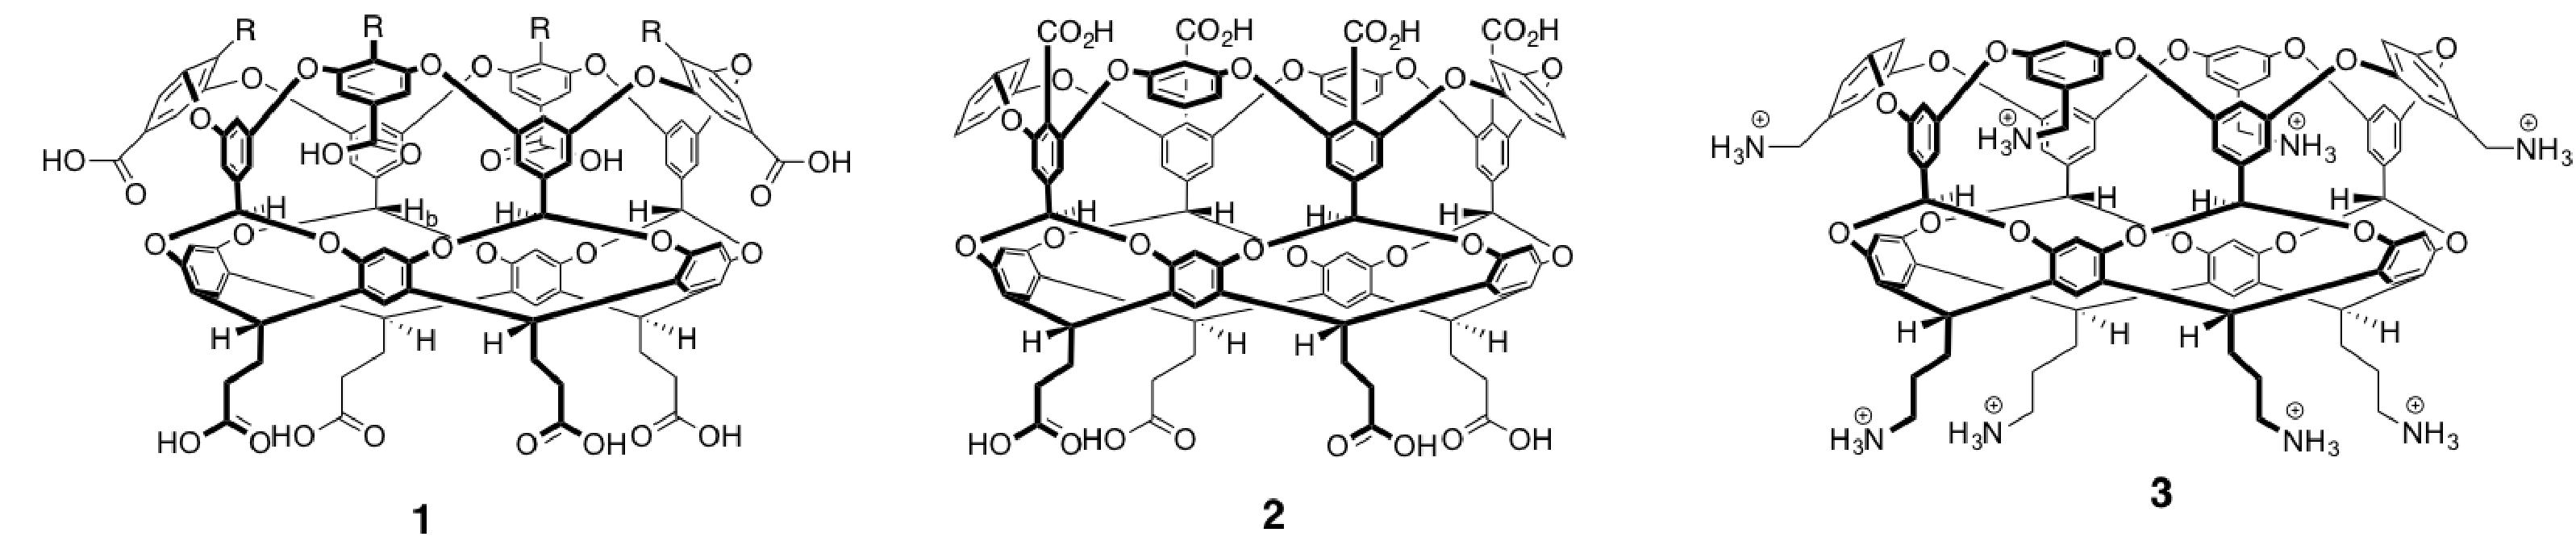
\includegraphics{figures/gdccs.pdf}}

\end{centering}

\vspace{0.1in}
\caption{\footnotesize {\bf Gibb deep cavity cavitands for SAMPL6-10.} These hosts bind a variety of carboxylate and trimethylammonium guests in a strongly salt-dependent manner, providing a stringent test of our ability to model binding and how it depends on these effects.
\label{figure:gdccs}}
\end{figure}

{\bf Novel deep cavity hosts probe the effects of binding site charge constellations.} 
For future SAMPL challenges, we will expand on the range of hosts by including {\bf 2} and {\bf 3} in our ITC studies (Figure~\ref{figure:gdccs}).  
Like cavitand {\bf 1}, host {\bf 2} is an octa-acid derivative.  However, the four benzoate groups are relocated from the extreme exterior in the case of {\bf 1}, to the rim of the binding pocket in {\bf 2}.  
We surmise that this will have a direct effect on the binding of charged guests as well as an indirect effect on guest complexation via changes to the solvation of the empty host.  
Octa-trimethylammonuim cavitand (``positand'' {\bf 3}) has the same overall architecture as host {\bf 1}, but inverts the charges on the water solubilizing exterior coat.  
While it is not yet clear if this switch in groups relatively remote from the pocket will directly affect guest complexation, results from related systems suggest it can (unpublished). 

{\bf SAMPL6-10 deep cavity cavitand challenges.} 
SAMPL6 will focus on how well the effect of host carboxylate substituent location can be predicted, and will involve hosts {\bf 1} and {\bf 2} with a set of five previously uninvestigated guests.  
Guests will be selected from commercial sources on the basis of reference calculations in a similar manner to SAMPL7 in Subaim 2.1, specifically picking guests which have broad dynamic range and, here, have marked differences in affinities between hosts.
SAMPL7 will provide a second iteration of this experiment to test algorithmic improvements in predictive modeling following SAMPL6 by comparing hosts {\bf 1} and {\bf 3} with a different set of guests.  
We anticipate that because of the relative remoteness of the charged groups in these two hosts, the effects of switching charges will be subtler than the differences between {\bf 1} and {\bf 2}.  
SAMPL8 will consider the effect of common biologically-relevant counterions/salts salts on guest binding, comparing the effects of NaCl and NaI on the complexation of five guests to {\bf 1}.  
We have previously shown that iodide has a weak affinity for the binding pocket of {\bf 1}, while sodium ions have an affinity for the outer carboxylates~\cite{carnegie_anion_2014}, requiring modeling to capture the differential affinities of these ions in addition to guest affinities to successfully model the observed affinities.  
SAMPL9 will follow up on this by examining the effects of these same two salts on the complexation of five guests to {\bf 3}, again giving the modeling community time to incorporate algorithmic improvements following SAMPL8. 
While we have not yet quantified salt affinities to host {\bf 3}, we expect the iodide to have affinity for both the pocket and the positively charged solubilizing groups.  
For SAMPL10 we will consider the effects of co-solvents on the binding of five guests to {\bf 1} and {\bf 2} to probe the effect of co-solvent competition for the binding site, as well as effects cosolvents may have in weakening the hydrophobic effect. 
%* I'm a bit concerned that proposing to measure only five ligands per compound is going to be perceived as lacking in statistical power required to assess accuracy, and that this specific aspect will be a liability. Is it possible to do more than that, or would this require a significantly larger chunk of money or access to automated ITC technology? Alternatively, we can be vague about how many compounds we will use or focus on the total number of compounds across all hosts. (DLM: I should probably recast a bit somewhere to explain how much we'll learn across hosts. Here:)
While the number of guests considered in each challenge is relatively small, the total number of binding affinities measured is significant across the full family of hosts, meaning that the full data set will be of considerable value as a benchmark set~\cite{mobley_predicting_2016}. 


%Aim 3 - Generate biologically relevant advanced model systems for protein-ligand binding challenges. (2 pages) 
%{\bf Aim 3. Generate biologically relevant advanced model systems for protein-ligand binding challenges.}
\textbf{\underline{Aim 3}: Develop model protein-ligand systems that isolate specific modeling challenges of drug targets.}
We seek to drive advances in quantitative modeling of protein-ligand interactions.
While D3R~\cite{gathiaka_d3r_2016} benchmarks accuracy for targets of pharmaceutical interest, it does not provide a clear route to improving poor performance because the large number complexities exhibited by these targets make it difficult to identify clear points of failure~\cite{ignjatovic_binding-affinity_2016, deng_large_2016, sunseri_d3r_2016, gathiaka_d3r_2016}.
For example, while kinases are targets of great interest to drug discovery, blind challenges involving kinase targets conflate issues of slow protein conformational dynamics~\cite{Lin:2013:Proc.Natl.Acad.Sci.}, protonation state effects of both protein~\cite{Shan:2009:PNAS} and ligand~\cite{Szakacs:2005:JournalofMedicinalChemistry,Grante:2014:SpectrochimicaActaPartA:MolecularandBiomolecularSpectroscopy}, charged ligands, and the modeling of complex divalent salt environments and phosphorylation state effects along with the standard challenges of conformational sampling and forcefield accuracy.
Thus D3R exercises serve the community well to understand current accuracy, but {\bf blind challenges on complex pharmaceutical targets have limited ability to rapidly advance quantitative predictive modeling.}

%%%%%%%%%%%%%%%%%%%%%%%%%%%%%%%%%%%%%%%%%%%%%%%%%%%%%%%%%%%%%%%%%%%%%%%%%%%%%%%%
% FIGURE: HSA SAMPL6 CHALLENGE
%%%%%%%%%%%%%%%%%%%%%%%%%%%%%%%%%%%%%%%%%%%%%%%%%%%%%%%%%%%%%%%%%%%%%%%%%%%%%%%%
\begin{figure}[h]
\begin{centering}
\resizebox{\textwidth}{!}{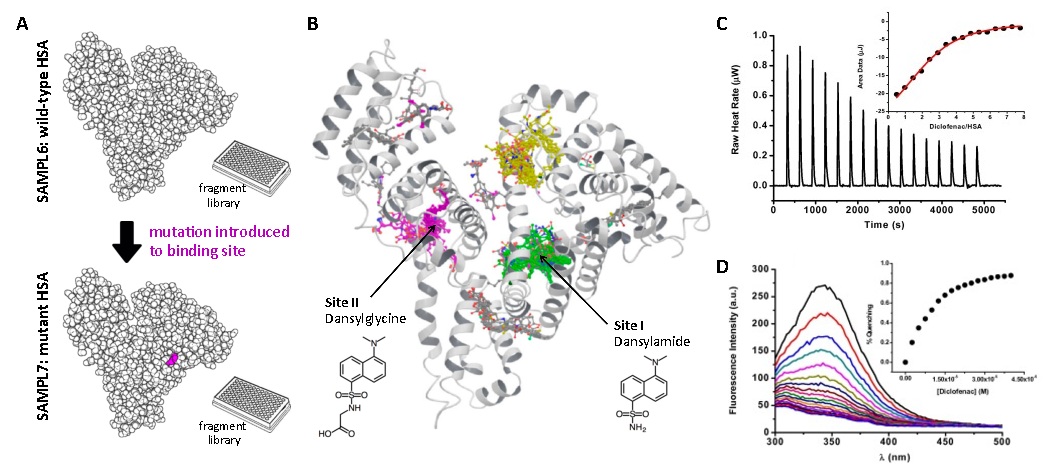
\includegraphics{figures/hsa-figure-draft4.pdf}}

\end{centering}
\vspace{0.1in}
\caption{\footnotesize {\bf The SAMPL6/7 protein-ligand challenge focuses on soluble drug fragment binding to human serum albumin (HSA).}
\emph{(A)}~SAMPL6 will study binding of a library of 96 small soluble drug fragments to recombinant HSA.
We will introduce a mutation in one of the binding pockets to create a challenge target for SAMPL7.
\emph{(B)}~HSA has at least eight known binding sites, with major well-characterized sites (green, Sudlow's Site I; purple, Sudlow's Site II) which bind a variety of drugs%, often modulating their pharmacokinetics~\cite{Fasano:2005:IUBMBLife(InternationalUnionofBiochemistryandMolecularBiology:Life)} 
(figure from~\cite{Hall:2013:JournalofChemicalInformationandModeling}).
%DLM: Is the pharmacokinetics aspect relevant/important here? (Cutting for now since (a) this is also stated in the text, and (b) doesn't seem that relevant here)
Two fluorescent probes---dansylamide and dansylglycine---have been shown to bind with $\sim$$\mu$M affinity and high selectivity to Site I and Site II, respectively; both exhibit binding-enhanced fluorescence at 480 nm, and can be used to site-specifically probe ligand affinities by competition.
\emph{(C)}~Binding affinities of soluble molecules can easily be measured by isothermal titration calorimetry (ITC); here, the ITC titration of HSA by diclofenac (a Site II ligand~\cite{Rafols:2014:Talanta}) is shown~\cite{Bou-Abdallah:2016:TheJournalofChemicalThermodynamics}. 
\emph{(D)}~HSA tryptophan fluorescence quenching can also be used to measure ligand binding affinity; here, HSA titration by diclofenac is shown, with the inset plot showing percent quenching at 346 nm~\cite{Epps:1999:JournalofPharmacyandPharmacology,Bou-Abdallah:2016:TheJournalofChemicalThermodynamics}
\label{figure:hsa-challenge}}
\end{figure}
%%%%%%%%%%%%%%%%%%%%%%%%%%%%%%%%%%%%%%%%%%%%%%%%%%%%%%%%%%%%%%%%%%%%%%%%%%%%%%%%

{\bf We take the alternative approach of identifying and developing specific protein-ligand systems which \emph{isolate} individual accuracy-limiting effects in a series of prospective challenges.}
By developing \emph{model binding systems}---real protein-ligand systems that may be of pharmacological interest, but comprised of single-domain proteins binding to a simple ligand series free of complex phenomena---we can study systems of complexity intermediate between completely artificial systems (such as the T4 lysozyme L99A system developed by Shoichet and Matthews~\cite{mobley_predicting_2007,merski_homologous_2015, mobley_predicting_2016}) and complex pharmaceutical targets where multiple modeling challenges make it difficult to learn from failure (Figure~\ref{figure:mining-for-model-systems}A).
This process focuses the field on identifying and evaluating multiple solutions to selected accuracy-limiting effects (such as how to deal with ligand and protein protonation-state issues~\cite{Onufriev:2013:QuarterlyReviewsofBiophysics}, slow protein conformational dynamics, etc.) while avoiding other complicating factors.

While model systems have had ample success in driving progress in individual research laboratories, community participation in blind challenges amplifies their power.
For example, SAMPL3 featured the binding of small, rigid charged molecules to bovine trypsin~\cite{Newman:2011:JComputAidedMolDes}, and rapidly focused the field on the deficiencies of current alchemical free energy methodologies in treating the binding of charged ligands.
Within two years, multiple laboratories had developed practical solutions to effectively handle charged ligand binding~\cite{Rocklin:2013:TheJournalofChemicalPhysics, lin_overview_2014, Reif:2014:JournalofComputationalChemistry}.

{\bf SAMPL6-10 model protein-ligand challenges.} 
We will introduce a new model protein-ligand system each year, with challenges fielded for each system for at least two consecutive years to allow iterative methodology improvement and assessment.
%Immediately following the challenge, the data (including all primary data) will be published and released as a version-controlled benchmark dataset for retrospective evaluation.
%DLM: That's a statement for Aim 4 (which we already have there); cutting.
Our SAMPL6 challenge will focus on binding of small soluble drug fragments to one particular protein (below). 
However, maximizing gains in this area requires adapting subsequent challenges based on deficiencies identified by the previous year's D3R/SAMPL challenges.
Therefore, subsequent model systems will be rapidly identified and developed using our new informatics platform for identifying tractable model systems.
%The above had material on HSA which was repeated in the immediately following paragraph, so I cut it.

{\bf SAMPL6: Assessing predictive modeling of binding to multiple weak sites via measuring fragment binding to human serum albumin (HSA).}
HSA, the most abundant blood plasma protein, has a remarkable ability to bind a great variety of small molecule drugs in multiple binding sites (Figure~\ref{figure:hsa-challenge}B)~\cite{Fasano:2005:IUBMBLife(InternationalUnionofBiochemistryandMolecularBiology:Life)}.
As a result, HSA not only helps isolate the challenge of multiple weak ligands binding to a stable rigid protein, but it is also a pharmacologically relevant because of how it drastically modulates drug pharmacokinetics~\cite{Hall:2013:JournalofChemicalInformationandModeling}.
HSA has at least \emph{eight} known binding sites, with numerous crystal structures available for drugs binding to two predominant sites (Sudlow Site I and II)~\cite{Hall:2013:JournalofChemicalInformationandModeling}.
Small soluble molecules resembling drug fragments are highly likely to bind to HSA ($\ge$90\% of such fragments, as detected by SPR~\cite{Elinder:2011:JournalofBiomolecularScreening}), providing an experimentally-tractable diverse set of ligands spanning several orders of magnitude in affinity~\cite{Elinder:2011:JournalofBiomolecularScreening}.
As current advanced methodologies such as alchemical free energy calculations currently assume a single well-defined binding site with high affinity~\cite{Gilson:1997:BiophysicalJournal}, this dataset will allow the isolation of the effect of weak multiple binding from the majority of other confounding factors in protein-ligand binding.
As HSA is relatively rigid, and computational methods already show some promise in computing binding affinities to HSA~\cite{Hall:2013:JournalofChemicalInformationandModeling,Lexa:2014:PLoSONE,Evoli:2016:bioRxiv}, this is an optimal model system for SAMPL6.

Recombinant HSA will be expressed in \emph{E.~coli} and purified via refolding from inclusion bodies~\cite{Latta:1987:Bio/Technology}, then defatted at low pH~\cite{Lang:2015:BiotechnologyProgress} to ensure the resulting protein is free of the glycosylation and bound fatty acids found in plasma-isolated HSA~\cite{Lang:2015:BiotechnologyProgress}.
Recombinant expression will also allow a mutant form of HSA (engineered via single-primer mutagenesis) to be fielded for SAMPL7 (Figure~\ref{figure:hsa-challenge}).
We will obtain a diverse library of 96 soluble drug-fragment-like molecules in pre-plated format as dry compound, and assay it for HSA binding using automated isothermal titration calorimetry (ITC) (Figure~\ref{figure:hsa-challenge}C) to characterize the overall binding affinity of each compound to HSA.
The same ligands pre-plated in DMSO format will be used to conduct a separate set of fluorescence titration assays (monitoring tryptophan fluorescence quenching, Figure~\ref{figure:hsa-challenge}D) and competition assays in which the site-specific fluorescent probes daynsylamide (Site I) and dansylglycine (Site II) will be used to measure site-specific affinities for Sites I and II (Figure~\ref{figure:hsa-challenge}B), allowing participants to validate binding site predictions and site-specific affinity.
%Remove redundancy between this paragraph and the caption to save space? (i.e. refer to there for some of this content?)

%%%%%%%%%%%%%%%%%%%%%%%%%%%%%%%%%%%%%%%%%%%%%%%%%%%%%%%%%%%%%%%%%%%%%%%%%%%%%%%%
% FIGURE: MODEL SYSTEM MINING
%%%%%%%%%%%%%%%%%%%%%%%%%%%%%%%%%%%%%%%%%%%%%%%%%%%%%%%%%%%%%%%%%%%%%%%%%%%%%%%%
\begin{figure}[h]
\begin{centering}
\resizebox{!}{3in}{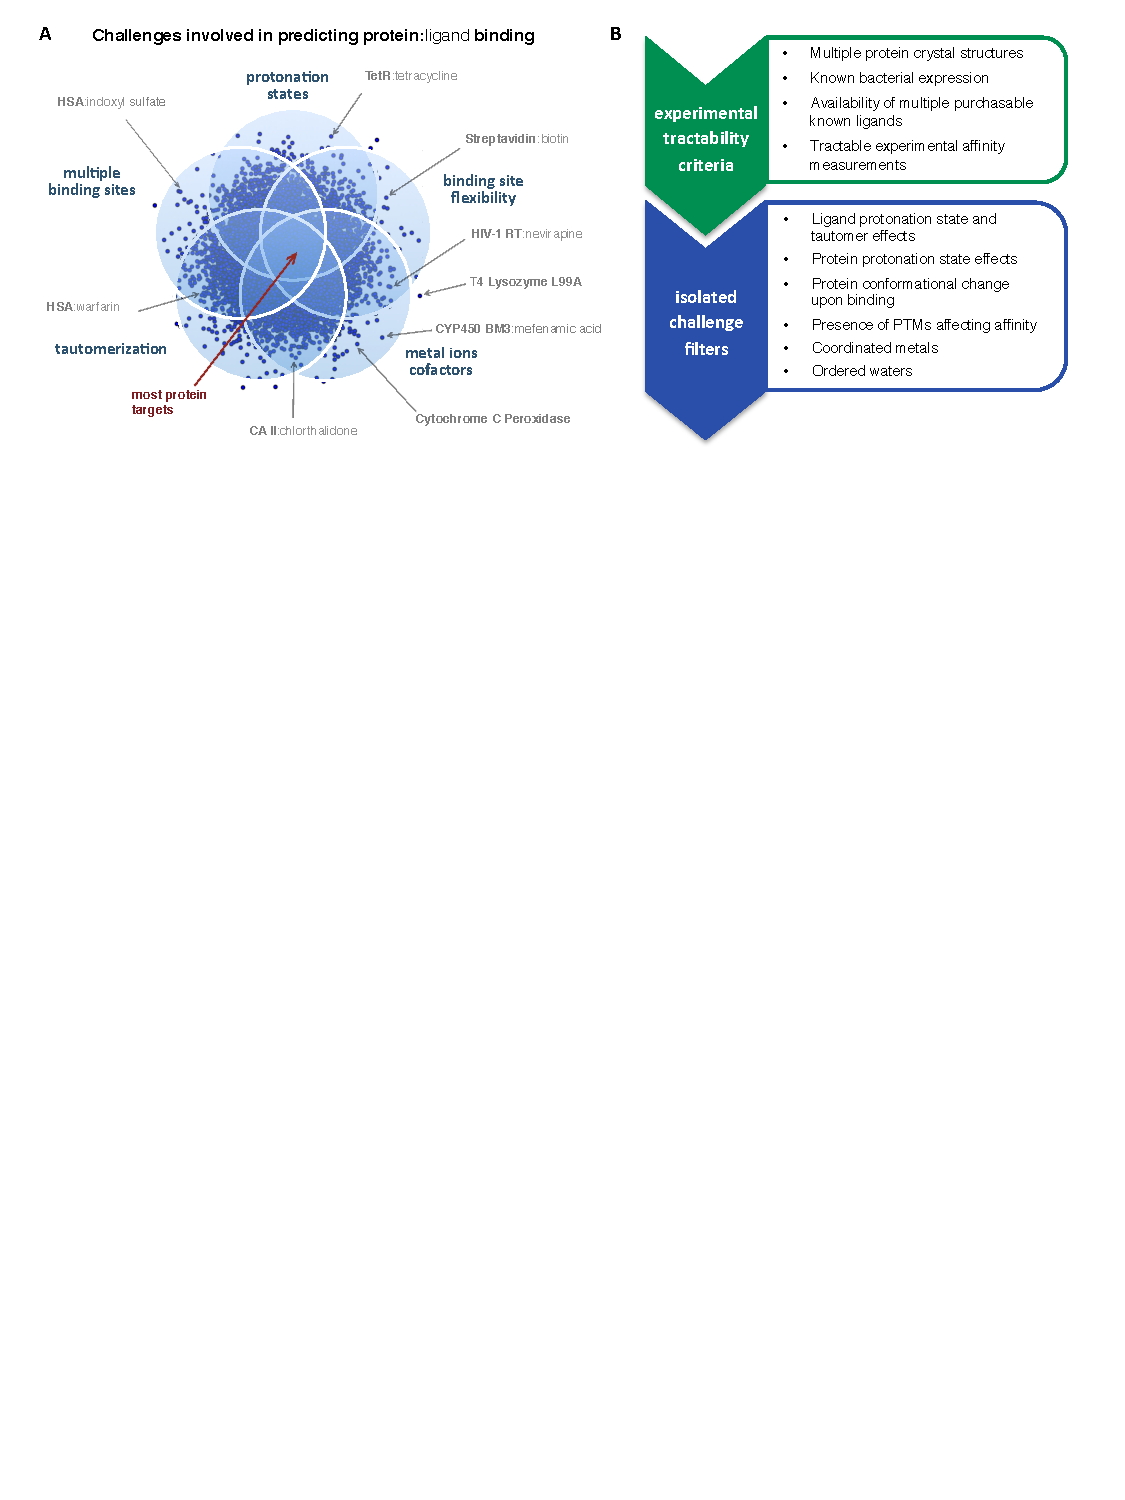
\includegraphics{figures/model-systems-figure-draft3.pdf}}

\end{centering}
\vspace{0.1in}
\caption{\footnotesize {\bf Mining model protein-ligand systems to focus on individual modeling challenges via a structural and chemical informatics platform.}
SAMPL7-10 will introduce protein-ligand systems selected to focus on individual challenges judged to be of critical immediate importance following current D3R/SAMPL blind competitions. 
\emph{(A)} Since most protein targets of pharmaceutical interest feature a multitude of simultaneous challenges, our goal is to identify model protein targets that isolate individual effects to guide modeling improvements. 
Some example protein-ligand pairs and the conceptual challenge categories they fall under are shown in the figure: 
T4 Lysozyme L99A~\cite{mobley_predicting_2007}, HSA~\cite{Martin:2009:JournalofComputer-AidedMolecularDesign}, Carbonic anhydrase II (CAII)~\cite{Martin:2009:JournalofComputer-AidedMolecularDesign,Temperini:2009:Bioorganic&MedicinalChemistry}, Cytochrome C Peroxidase~\cite{Rocklin:2013:JournalofMolecularBiology}, Cytochrome P450 BM3 M11 (CYP450 BM3)~\cite{Venkataraman:2014:Bioorganic&MedicinalChemistry}, HIV-1 Reverse Transcriptase (HIV-1 RT)~\cite{Gunasekaran:2007:JournalofMolecularBiology,Khunnawutmanotham:2009:BeilsteinJournalofOrganicChemistry}, Streptavidin~\cite{Gunasekaran:2007:JournalofMolecularBiology}, Tet repressor protein (TetR)~\cite{Gunasekaran:2007:JournalofMolecularBiology,Aleksandrov:2007:ChemBioChem}.
\emph{(B)} In order to rapidly identify and develop these tractable new model protein-ligand systems, we are developing a structural and chemical informatics system called TargetExplorer [\url{https://github.com/choderalab/targetexplorer}] that applies successive filters to all potential protein-ligand systems for which structural data is available. 
Suitable model systems should meet all experimental tractability criteria (green box) and possess only a few challenging properties, ideally only one (blue box).
\vspace{-0.1in}
\label{figure:mining-for-model-systems}}
\end{figure}
%%%%%%%%%%%%%%%%%%%%%%%%%%%%%%%%%%%%%%%%%%%%%%%%%%%%%%%%%%%%%%%%%%%%%%%%%%%%%%%%

{\bf SAMPL7-10: Rapid, responsive development of new model systems using a novel informatics platform.}
We are developing a novel informatics platform (TargetExplorer) aimed at identifying protein targets that can be rapidly developed into experimentally- and computationally-tractable model systems focusing on individual challenges (Figure~\ref{figure:mining-for-model-systems}).
This tool filters all known protein targets with structural data available in the PDB, first selecting for experimental tractability, then annotating experimentally tractable targets to determine which targets possess (or are likely to be free of) specific challenges for physical modeling (Figure~\ref{figure:mining-for-model-systems}B).
This will allow us to select systems which introduce only specific modeling challeges.
%We will make this tool accessible to other laboratories via a web interface during the course of this project.
%DLM: Cutting because we say below our tools will be available open source, and I don't think the web interface aspect is going to be a major selling point

Experimental tractability includes: (1) the availability of multiple protein crystal structures with at least one ligand-bound structure; (2) known bacterial expression (e.g.~from PDB {\tt EXPRESSION\_SYSTEM} records); (3) binding to a wide dynamic range of ligands (determined via data available in ChEMBL); (4) the availability of multiple known purchasable ligands (via ZINC); (5) tractability of experimental affinity measurements, such as known ligands with potentially fluorescent scaffolds (for fluorescence competition assays), highly soluble ligands (for ITC), or ligands above a minimal mass (for SPR or MST).
A number of additional filters annotate experimentally tractable systems with their potential computational challenges, such as: charged ligands or potential ligand protonation state or tautomer effects~\cite{Martin:2009:JournalofComputer-AidedMolecularDesign} (deduced from predicted aqueous protonation/tautomer energies); potential protein protonation state effects (deduced from MCCE2 calculations~\cite{Song:2009:JournalofComputationalChemistry}); protein conformational changes (deduced from variation in protein conformation or the presence of unresolved loops in protein-ligand crystal structures); the presence of post-translational modifications that may affect affinity (deduced from Uniprot annotations); coordinated metals (identified in crystal structures); ordered waters (present in multiple crystal structures); etc.

The Chodera lab has developed an automated wetlab specifically to develop such model protein-ligand systems using bacterial expression techniques (see Equipment and Facilities).
Potential targets matching desired challenge criteria will be screened for bacterial expression using high-throughput cloning, transformation, and expression testing, with purity and yield assessed by capillary electrophoresis on a Caliper GXII.
Targets will be screened for stability in various buffers using Thermofluor thermal shift assays~\cite{Reinhard:2013:ActaCrystallographicaSectionFStructuralBiologyandCrystallizationCommunications}.
Ligands identified via TargetExplorer as spanning a wide dynamic range of binding affinities will be purchased as dry powder stocks and prepared for assay by highly accurate gravimetric solution preparation techniques using a Quantos automated balance.
Our lab has access to a wide variety of biophysical techniques for quantitative measurement of protein-ligand binding affinities, including fluorescence (if fluorescent probe ligands are available), absorption (e.g.~Soret band shifts), automated isothermal titration calorimetry (provided ligands are sufficiently soluble), surface plasmon resonance, microscale thermophoresis (MST), luminescence, and alphascreen; all except MST are fully automated. 

We take a twofold approach to developing challenge datasets:
First, we will purchase and assay small molecules similar to known ligands, presuming that these molecules are likely to have measurable affinities.
Second, using single-primer quick-change mutagenesis, we will introduce site-directed mutants to modulate the binding affinities of known ligands.
This can be performed and screened for expression in 96-well format.
Thus, datasets will consist of a matrix of protein mutants and ligands, providing opportunity to deeply explore the effects of interest.


%Aim 4 - Coordinate, run, and analyze blind challenges to advance modeling of binding (1.5 pages)
%{\bf Aim 4. Coordinate, run, and analyze blind challenges to rapidly drive progress in quantitative physical modeling.}
{\bf \underline{Aim 4}: Field iterated community blind challenges to advance quantitative biomolecular design.}
The value of the targeted datasets generated in Aims 1--3 will be amplified enormously by the strategic release of this data through multiple iterations of coordinated SAMPL blind challenges and related activities.
These blind challenges are designed to test the state of the art, provoke new methodological and force field innovations, allow comparative evaluation of methods, and drive downstream improvements.
The new, progressive, targeted nature of the data generated means that SAMPL challenges will now build on one another, and for success in later challenges, participants must build on lessons learned from prior challenges.
SAMPL challenges and subsequent data release activities will therefore facilitate rapid cycles of application, learning, and improvement.

{\bf SAMPL blind challenges.} Challenges will have yearly submission deadlines.
The full timeline for SAMPL challenges (Figure~\ref{figure:timeline}) will be made available on the SAMPL website [\url{https://drugdesigndata.org/about/sampl}] at the outset, allowing participants to plan their work and select what challenges to be involved in.
%{\color{red}[JDC: Historically, how many participants have we had? How many do we expect? Can we communicate how many researchers this has impacted even \emph{before} funding?]}
%Will try for a small figure on this
As experimental data for each component becomes available and is curated, input files and challenge details will be made available online (and advertise via e-mail lists from prior SAMPLs and CCL), at least six months prior to the challenge deadline; data not yet available at that time will be held for a subsequent challenge (with the exception of three months for year 1 due to startup timescales).
As in prior SAMPLs, submissions will be handled by a web upload service on the SAMPL website (which will be migrated to separate hosting if the D3R effort is not renewed) which validates submissions to ensure that they meet format standards we specify along with the challenge details. 
As in SAMPL4 and SAMPL5, analysis will also be conducted by our automated Python framework, and results will be returned automatically via a web framework.
%Participants will be allowed to submit multiple sets of predictions per SAMPL component to allow for comparative assessment of models.
%One new ingredient will be that each participant will be required to designate one submission as their ``primary'' submission which will be included in the formal ranking of performance; other submissions will still be analyzed and receive an assessment of performance, but only one will be formally ranked.
%We find that participants learn a great deal from being able to compare multiple methods or protocols, but providing some participants with more ``shots on goal'' than others in the formal ranking can be seen by some as unfair.
%Unnecessary details above.
All participant submissions and methodology descriptions will (as before) be made available publicly on the website, along with participant information (except for participants who specifically request to remain anonymous prior to submission).
Aggregate statistics and historical performance will also be made available on our website, along with a record of linking publications to historical submissions.

%Coordinate and run SAMPL blind challenges
\textbf{Our goal is not just to run blind challenges, but to advance modeling by helping participants identify both modeling failures and potential solutions.} 
To achieve this, we provide guidance to participants as to what known modeling issues we expect may be relevant when providing details on each SAMPL component.
For a host-guest system, for example, we might highlight known buffer/salt effects, protonation state challenges, and point out previous work on sampling challenges, with pointers to the relevant experimental work and to modeling work from past SAMPL challenges and elsewhere~\cite{mobley_predicting_2016}.
This helps participants design their approach.
%Run reference calculations to:
{\bf Additionally, we will run reference calculations using current best practices.} 
This serves several purposes:
		%a. Test current standard methods/FF
It provides a test of the current methods and force fields we select; 
		%b. Facilitate others learning (swap method or FF)
it helps facilitate learning---we announce what calculations we plan to perform, make input files available in a wide variety of formats~\cite{shirts_lessons_2016, yin_overview_2016, bannan_blind_2016}, and others can repeat our calculations with a different method but same system and force field to compare methods, or swap force field but keep the method and system fixed to compare force fields, etc.; 
		%c. Do sensitivity analysis (learn what?s important)
and it allows us to conduct sensitivity analysis, as by varying the conditions of our simulations (protonation state, tautomer, etc.,~\cite{bannan_blind_2016}) we can see how much this impacts calculated values and thereby how important it is, even if participants don't do these tests.
		%d. (Give examples of what we've learned from this)
Reference calculations have, for example, helped us highlight the importance of a small amount of water in cyclohexane for accurately calculating log D values, show how an incorrect tautomer could affect calculated values by many log units~\cite{bannan_blind_2016}, and discover that small forcefield modifications could significantly improve results on hydration free energies~\cite{mobley_blind_2014-1}.
		%e. (We will make inputs, outputs, and methods available too)
To further aid follow-up studies, we will make the input files, results, and simulation workflows used for our reference calculations---along with the data---available via GitHub and Docker Hub.


%Select and announce null models, run them
Physical methods are only valuable if they can reliably outperform alternate methods, so \textbf{a new focus of SAMPL6-10 will be selecting quality null models and running them to provide a point of comparison for participants}.
While SAMPL efforts in the past have used some null models, lack of manpower has required that these be particularly crude (such as ``guess zero'' models~\cite{bannan_blind_2016, paranahewage_predicting_2016, muddana_sampl4_2014}) which provide no predictive value. 
Null models will be announced when each challenge component is opened.
%Do statistical analysis of results (& compare to nulls), report back
Statistical analysis of SAMPL performance, and comparison with nulls, will continue to be an important component of our work.
%The paragraph above could probably be cut for space -- no one is going to fund us because we have great null models. May be better replaced by a figure.

%D3R coordination/meetings:
Following submission and analysis of each SAMPL challenge, challenge results will be released and discussed, with SAMPL workshops allowing more formal presentations on and discussion of results in years 1, 3, and 5. 
	%	a. Co-running workshops with D3R
Workshops will run every two years at the request of past participants, and will be co-run and co-hosted with D3R Grand Challenge workshops (see support letter).
During the off years, SAMPL challenges will still run, but discussion of and dissemination of results will be via asynchronous means (as discussed below) and a ``virtual workshop'' consisting of talks and interaction over Google Hangouts or YouTube Live.
	%     b. Coordinating challenges with them, submission deadlines offset from D3R challenges
While coordination with D3R will mostly be at the level of workshops, we will also ensure that SAMPL challenge submission deadlines are offset from D3R deadlines to allow maximum community participation in both efforts.

	%Coordinate with JCAMD on special issues
{\bf Dissemination of results and data.}
Rapid dissemination of results is critical so that new insights can be used in subsequent challenges.
We will continue to publish special issues of the \emph{Journal of Computer Aided Molecular Design} (JCAMD) collecting publications related to each year's SAMPL challenges (see Letter of Support).
	%Encourage prepublication sharing (bioRxiv) and sharing of slides/posters (F1000?)
To ensure immediate availability of reports, we will strongly encourage prepublication sharing of results and analysis, including both slides and posters from SAMPL meetings (via F1000 Research) and paper preprints (via bioRxiv).
	%Provide a way to connect up researchers to enable rapid progress, such as Slack
We also want to ensure that participants learn from one another by rapid exchange of ideas outside of formal workshops and meetings.
While this has happened in the past---for example, when participants using similar methods work together after the SAMPL meeting to identify the origin of these discrepancies~\cite{monroe_converging_2014, yin_overview_2016, bhakat_resolving_2016, bosisio_blinded_2016, mobley_predicting_2016}---we hope to accelerate this kind of collaboration.
To facilitate more open communication between the community, we will use collaboration software---such as Slack, which facilitates scientific communication for the NASA/JPL Mars Rover teams and NSF antarctic scientific research teams---to build a community discussion platform, 
facilitating a process of learning from one another more rapidly than normal publication channels.

%%%%%%%%%%%%%%%%%%%%%%%%%%%%%%%%%%%%%%%%%%%%%%%%%%%%%%%%%%%%%%%%%%%%%%%%%%%%%%%%
% FIGURE: TIMELINE
%%%%%%%%%%%%%%%%%%%%%%%%%%%%%%%%%%%%%%%%%%%%%%%%%%%%%%%%%%%%%%%%%%%%%%%%%%%%%%%%
\begin{figure}[h]
\begin{centering}
%\resizebox{!}{3.2in}{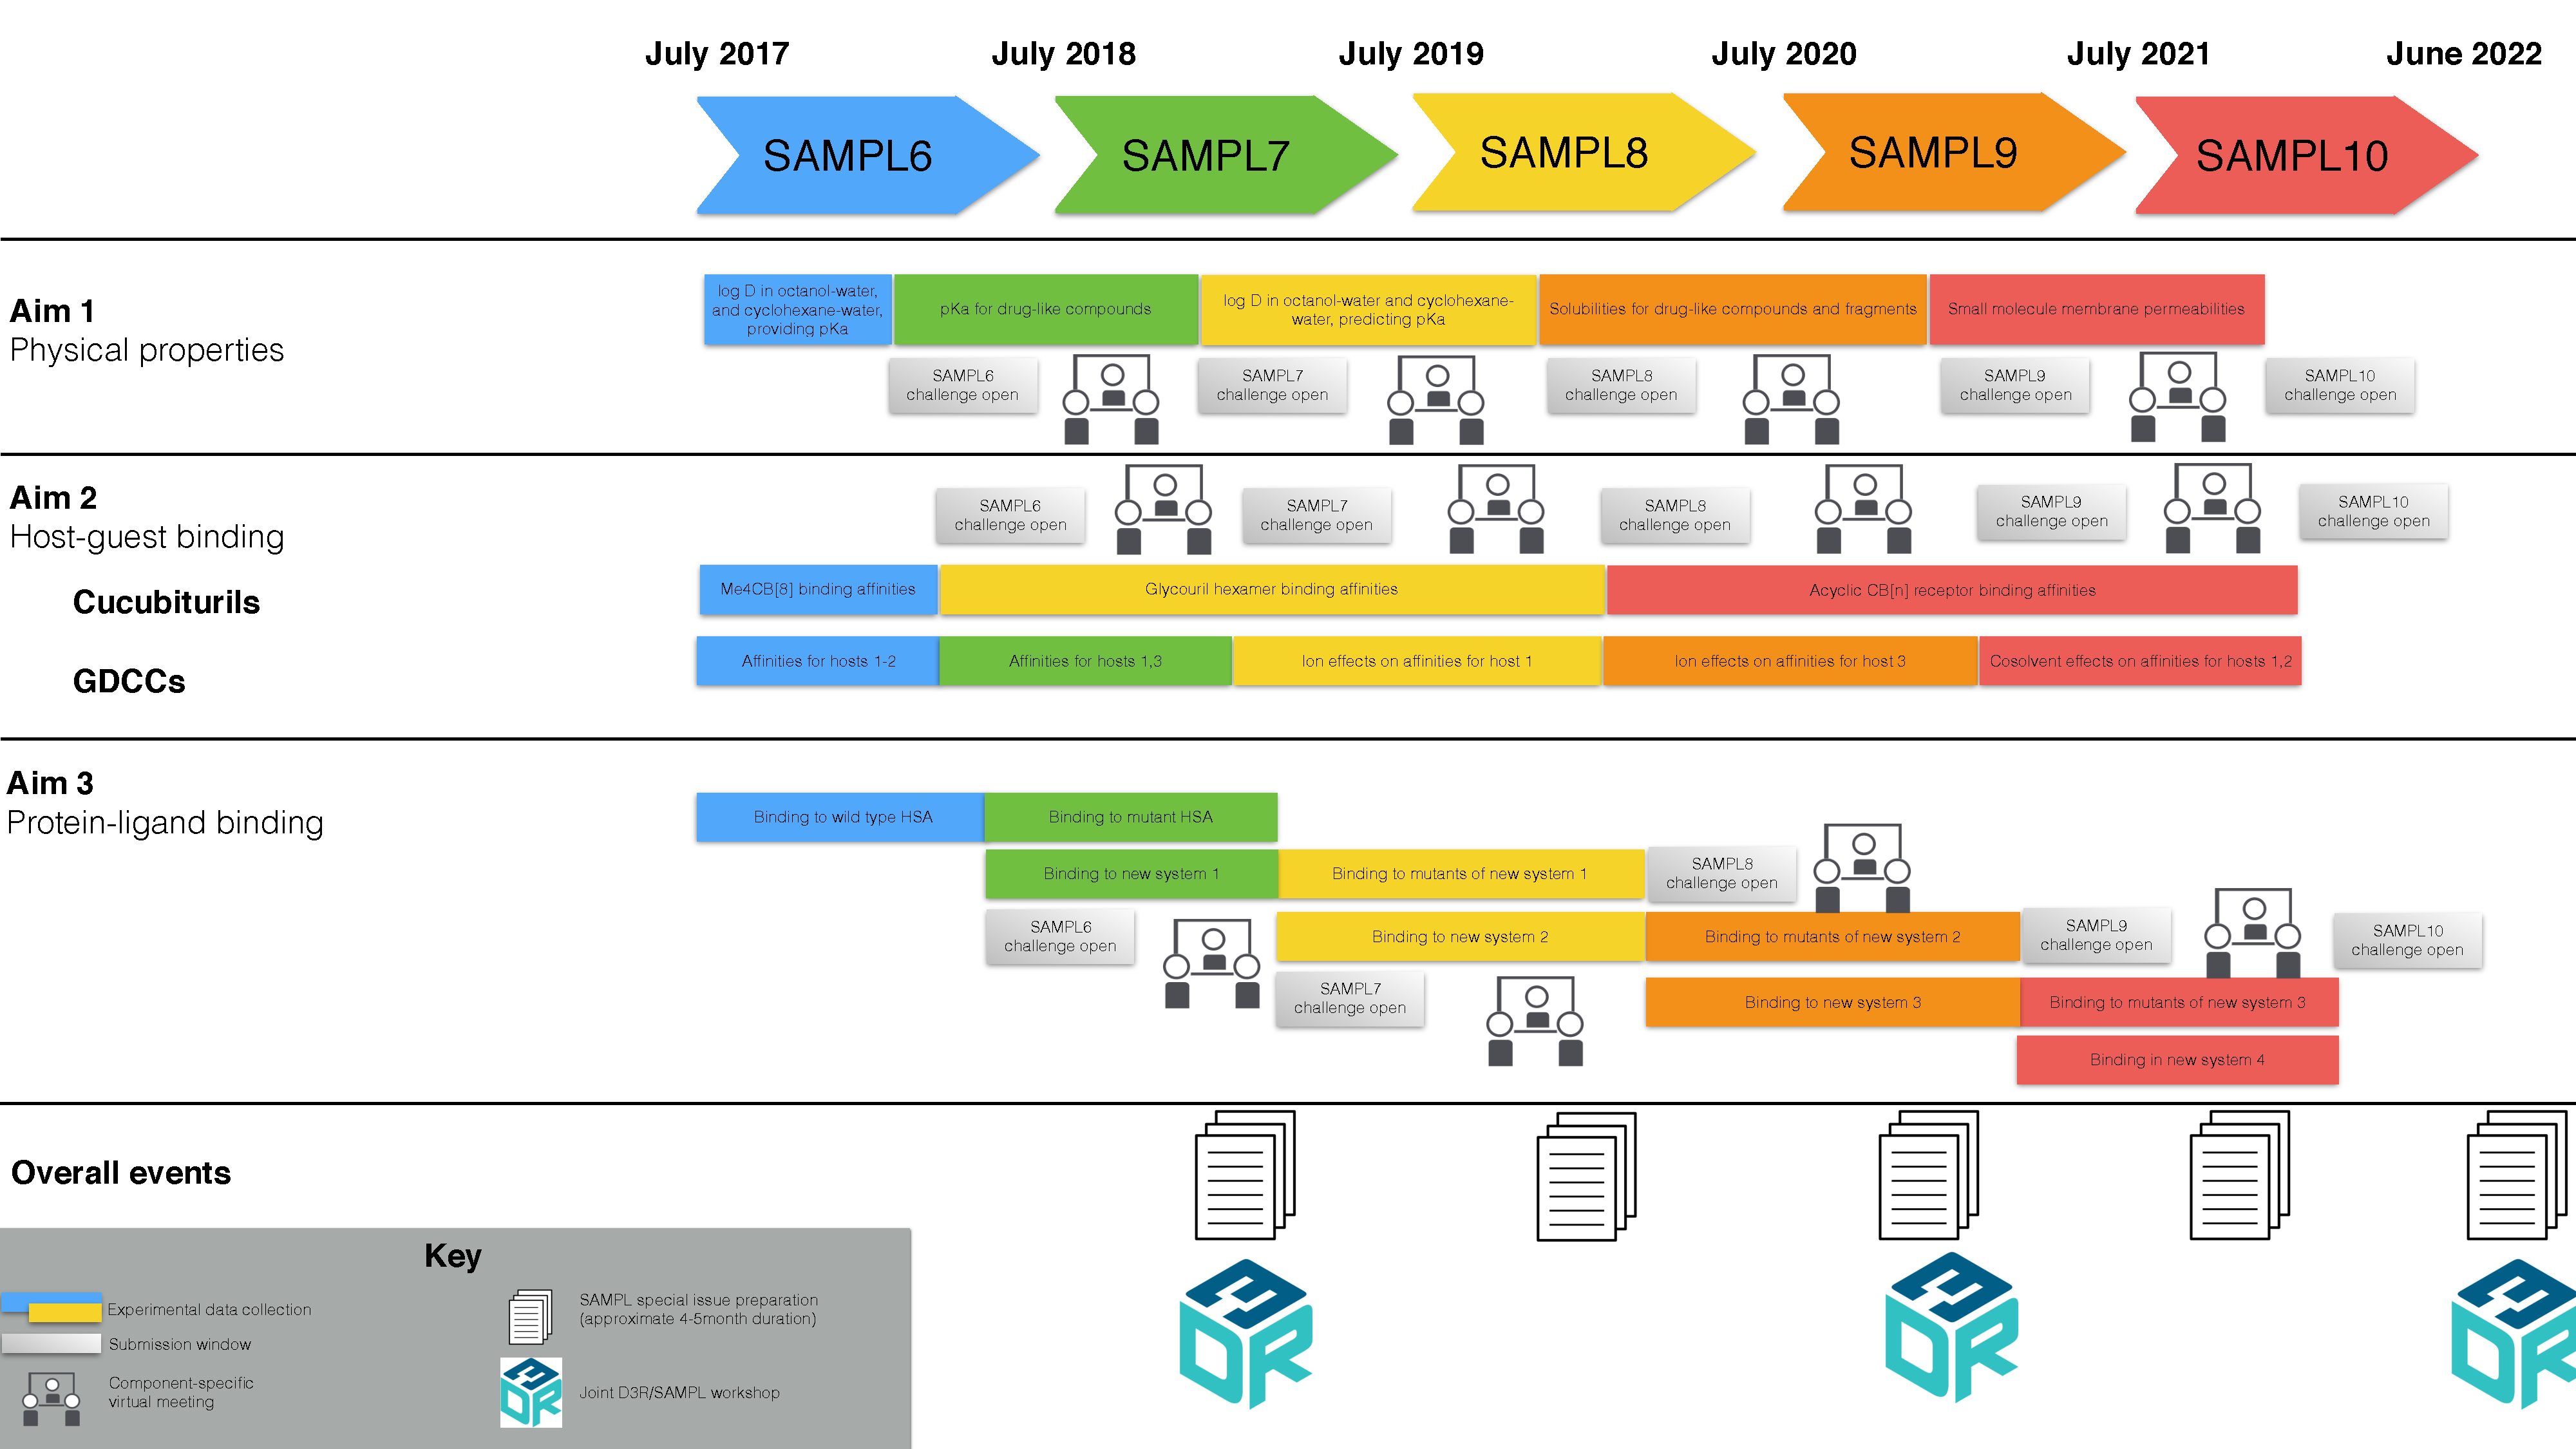
\includegraphics{figures/Timeline.pdf}}
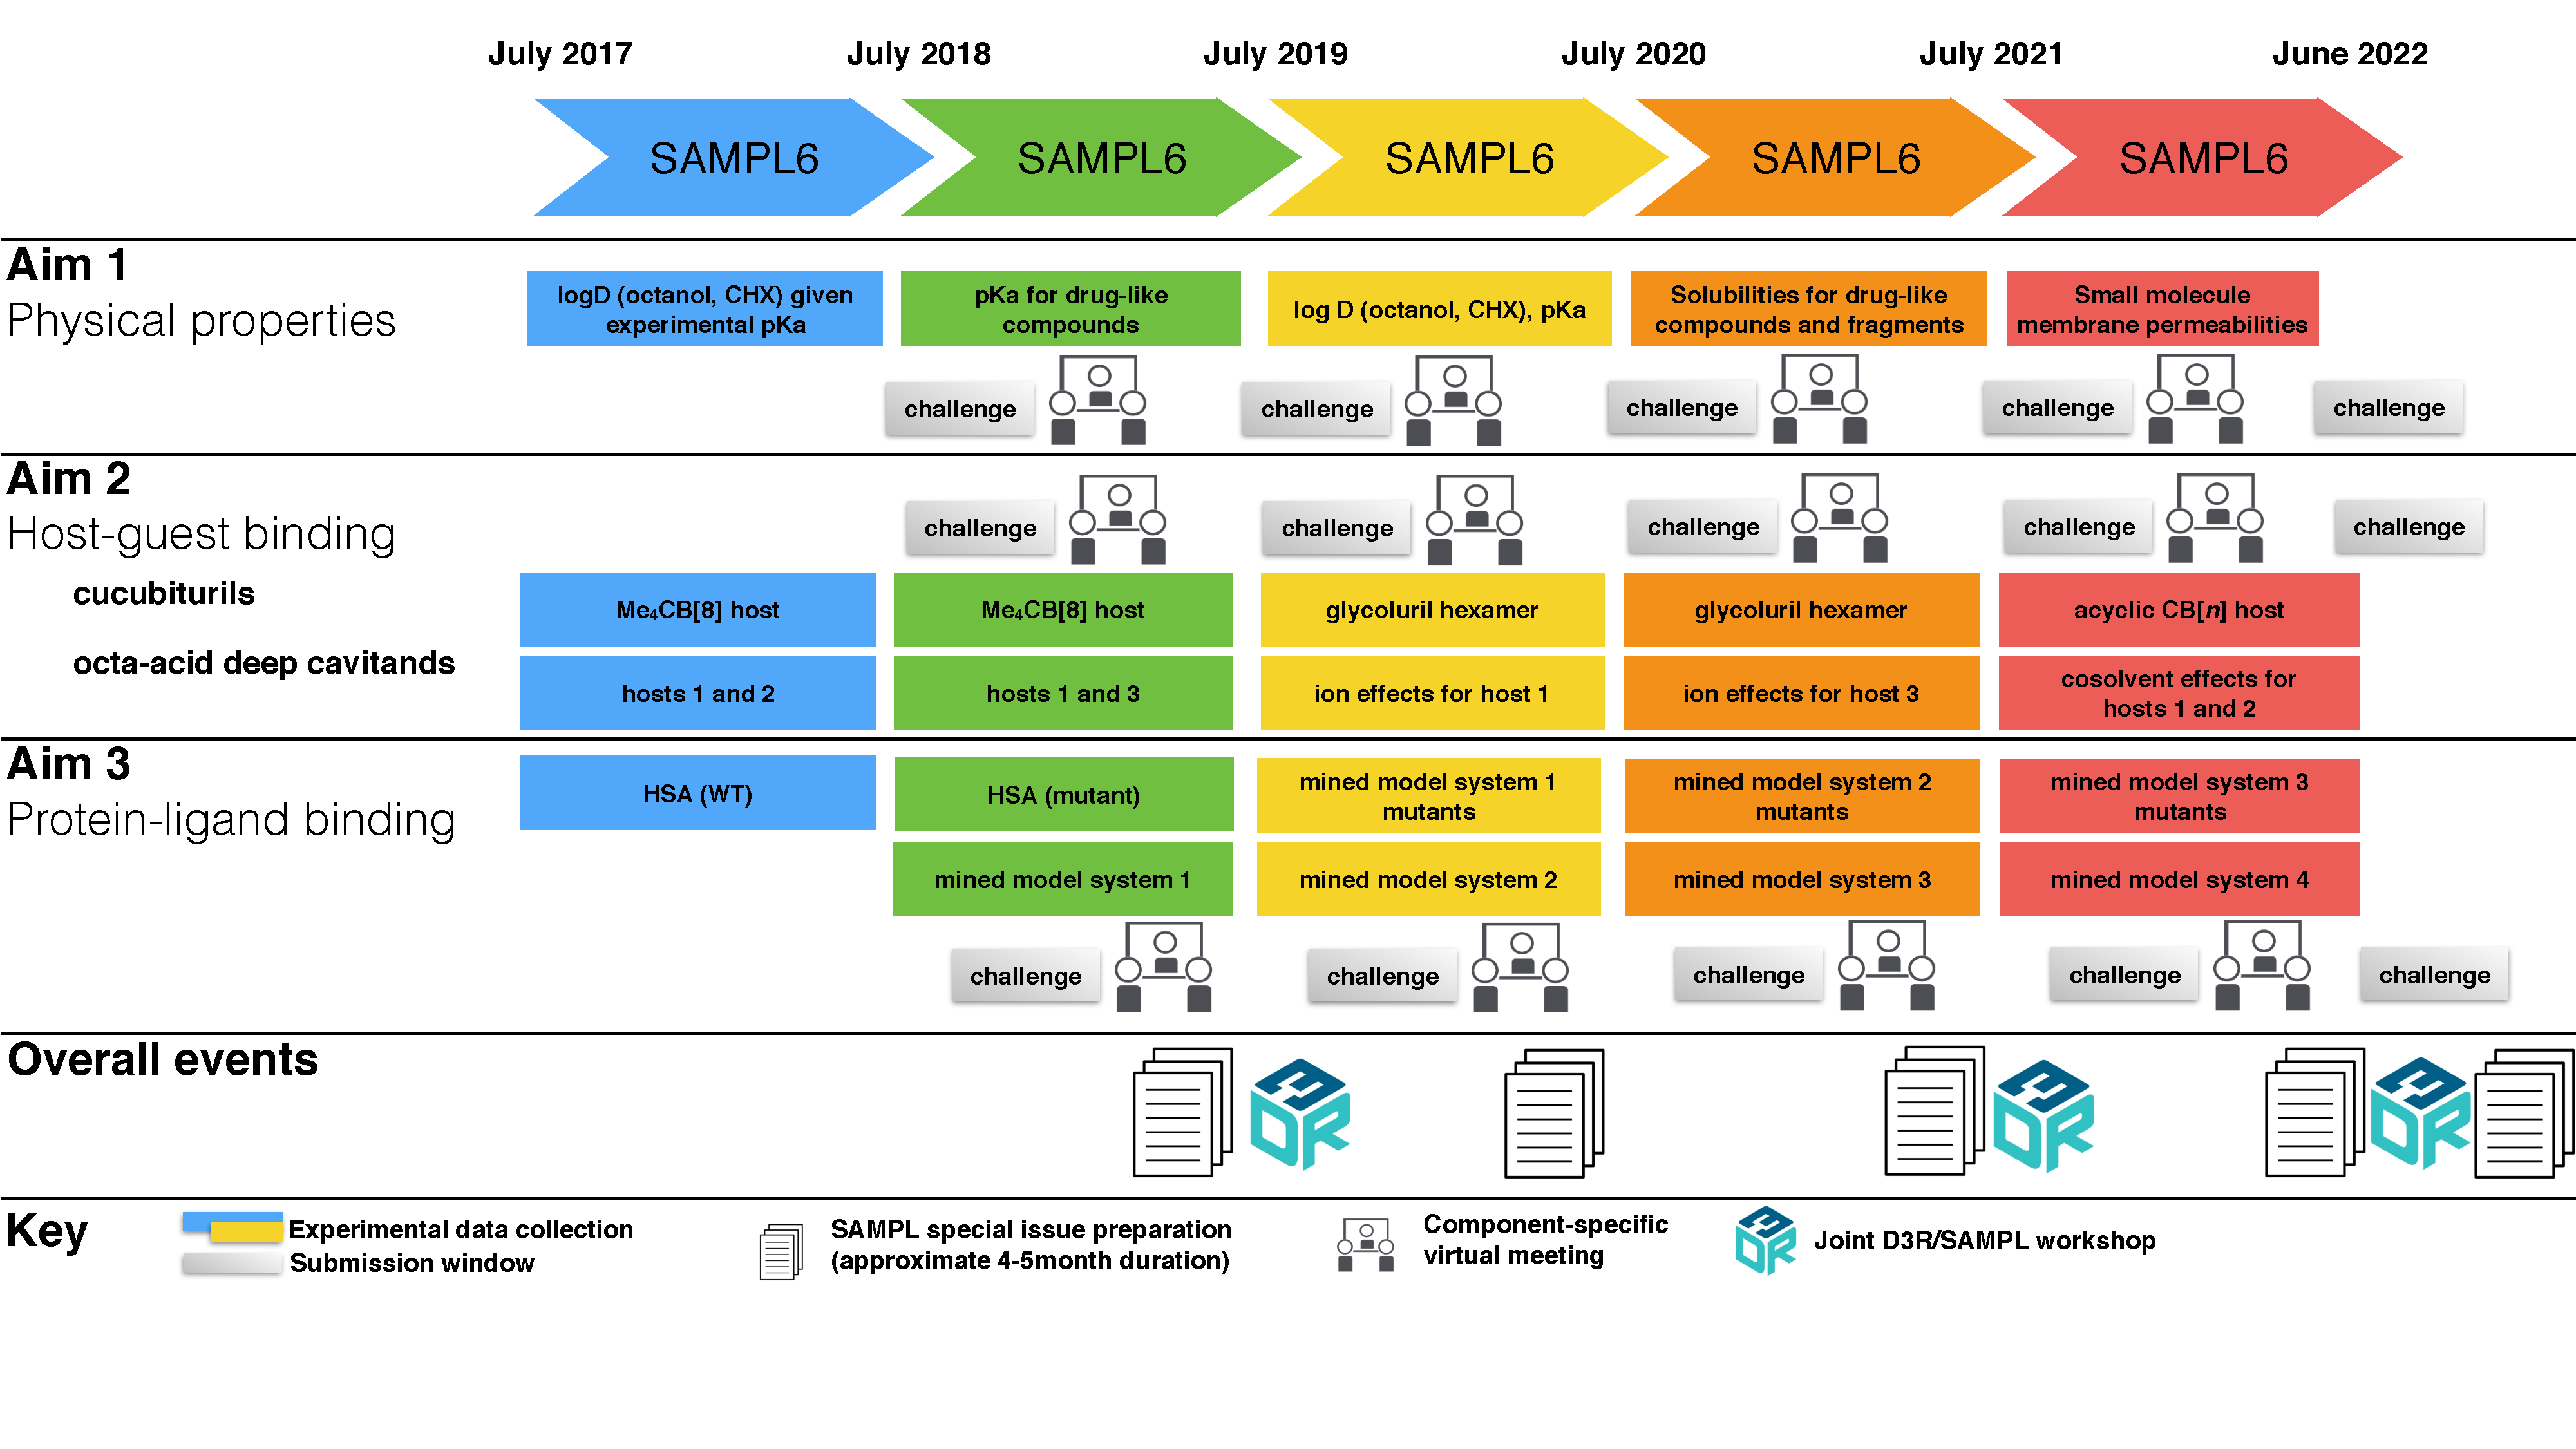
\includegraphics[width=\textwidth]{figures/Timeline2_cropped.pdf}
\end{centering}
\vspace{0.1in}
\caption{\footnotesize {\bf Timeline for our activities.} Activities covered by this grant include data collection and SAMPL challenges on our three major components (physical properties, host-guest binding, and protein-ligand binding), with each challenge cycle color-coded separately.  
Data collection within each Aim is shown by a colored bar indicating what is measured and curated.
Data collection/curation is followed by a submission window for that challenge component, then all results and analysis are returned to participants and posted on the SAMPL website; this also will nucleate more detailed discussion on the relevant Slack channel (which is expected to already be underway as participants prepare during the data collection phase). 
Each component will then wrap up with a focused virtual meeting where participants focus on lessons learned and areas which need further exploration; these will be recorded and posted on our website to assist in rapid dissemination of new insights. 
Virtual meetings precede the submission window for the next SAMPL challenge, giving participants the opportunity to incorporate lessons learned for the next challenge.
Submission windows and virtual meetings are staggered across categories so that participants can be involved in all three major areas without multiple simultaneous deadlines.
In-person meetings are co-hosted with D3R and will occur every two years.
Yearly special issues of JCAMD will have submission deadline shortly after the virtual meeting on the protein-ligand challenge for that year, and an approximate 4-5 month timeline (based on historical experience) from the submission deadline until the special issue appears (with the first papers appearing online substantially sooner).
Rapid dissemination of insights is critical for rapid progress, so we highly encourage the use of preprints and informal reports to supplement the special issue.
\label{figure:timeline}}
\end{figure}
%%%%%%%%%%%%%%%%%%%%%%%%%%%%%%%%%%%%%%%%%%%%%%%%%%%%%%%%%%%%%%%%%%%%%%%%%%%%%%%%

	%Data curation, archival and dissemination
\textbf{Each dataset will have a life cycle of collection, curation, blind challenges, and public dissemination}.
In the past, the unfunded nature of SAMPL has forced us to primarily emphasize the \emph{blind challenges} and pre-challenge \emph{curation} aspects, with isolated forays into collection~\cite{rustenburg_measuring_2016, Newman:2011:JComputAidedMolDes}. 
This work now considers the full life cycle, with Aims 1--3 dealing primarily with collection and pre-challenge curation.
Post-challenge, 
	%   Datasets will be curated and released as standard community benchmark datasets: For example, FreeSolv
datasets will receive additional curation, then be released as standard test or benchmark sets that allow retrospective evaluation of methodologies on high-quality data~\cite{mobley_predicting_2016}. 
The FreeSolv dataset, for example, includes a large number of calculated and experimental hydration free energies from SAMPL0--4, and provides a standard benchmark dataset for hydration free energy calculations~\cite{Mobley:2014:JComputAidedMolDes}.
	%   Data curation also via follow-up experiments (new!; cite examples where it was desirable)
Post-challenge curation will receive new attention here; in the past, lack of resources has always prevented follow-up experimental work, even when the data clearly indicated it was warranted (such as the puzzling issues with dynamic range for logD values in SAMPL5~\cite{rustenburg_measuring_2016, bannan_blind_2016}).
The requested budget will allow follow up experiments motivated by computation when warranted.
	%   Store and archive primary data and analysis
Dissemination is the final stage in the data life cycle (see Resource Sharing Plan); we will make the data (including primary data, processed data, and our analysis of challenge submissions) available freely and publicly with permanent, citeable DOIs; ensure relevant data is deposited in standard community repositories (e.g.~BindingDB~\cite{Liu:2007:Nucl.AcidsRes.}); and guarantee data longevity via backup hosting on library archival facilities (such as the UC's DASH (\url{https://dash.cdlib.org/})).

	%   Probably also should comment on archiving/disseminating OLD SAMPL data, which we haven't been able to do (lack of resources)
%Because prior SAMPL work focused mainly on challenges themselves, dissemination of the data has never been a major focus. As part of this project, we will retrieve old SAMPL experimental data, submissions, and analysis from where it is archived and make it available along with the new data generated here. 
%Cut the above for space. Won't excite anyone. We should do it -- but it's not going to make a difference in getting this funded.

	%   Methodology archival? Push for containerization of tools, maybe in conjunction with other known efforts. [Currently short on space, but putting something very short on this here anyway.]
We will also push for containerization of tools and methods in conjunction with other efforts such as AutoDesk's Molecular Design Toolkit and the NSF Molecular Sciences (MolSci) initiative.
Our vision is that long-term, instead of participants submitting a set of predictions, they would also submit the entire workflow they applied via Docker containers allowing reproducibility and repurposing, ensuring dissemination workflows, not just results.


%%%%%%%%%%%%%%%%%%%%%%%%%%%%%%%%%%%%%%%%%%%%%%%%%%%%%%%%%%%%%%%%%%%%%%%%%%%%%%%%%%%%%%%%%%%%%%%%%%%%%%
% COLLABORATION MANAGEMENT PLAN
%%%%%%%%%%%%%%%%%%%%%%%%%%%%%%%%%%%%%%%%%%%%%%%%%%%%%%%%%%%%%%%%%%%%%%%%%%%%%%%%%%%%%%%%%%%%%%%%%%%%%%

{\large \bf COLLABORATION MANAGEMENT PLAN} % 1 paragraph
% Collaboration history of success: Mobley and Chodera have worked together extensively in past SAMPL challenges and other areas; Mobley/Isaacs and Mobley/Gibbs have fielded past SAMPL challenges.
% PI Mobley will oversee entire project; Mobley/Chodera A1, Isaacs SA 2.1, Gibb 2.2, Chodera A3, Mobley/Chodera A4 (tapping other co-I as needed).
% How often will PI and co-Is talk/meet?
% Publication management plan.
% Conflict resolution plan.

We have a strong previous history of successful collaboration, with Mobley and Chodera having co-authored roughly a dozen publications since 2006, as well as several workshops and other initiatives.
Mobley, Isaacs, and Gibb have also worked together to coordinate past SAMPL challenges, and Mobley and Gibb a previous NSF workshop. 
PI Mobley will oversee the entire project, with Mobley and Chodera working together on Aim 1, Isaacs responsible for Aim 2.1, Gibb for Aim 2.2, and Chodera for Aim 3. Mobley and Chodera will conduct Aim 4, involving the other co-investigators as needed.
Meetings will consist of a Google Hangout monthly and a yearly in-person planning meeting.
Chodera and Mobley will communicate more frequently due to the interlinked nature of their work.
Publications are expected to be largely dictated by the overall Timeline, with an experimental publication associated with each challenge component being prepared for distribution to participants along with their results.
Conflict resolution is expected to be straightforward, but if any serious difficulties arise, Michael Gilson (UCSD) will be consulted as an arbiter, given the need this initiative has for close connections with D3R.

{\large \bf OUTLOOK} %or conclusions. 0.5 page
% This part is probably less critical, and can be dropped if space reasons dictate.

Physical methods have been slow to achieve their promise in binding prediction, in part because truly significant innovations are so hard to recognize due to a lack of standard tests and benchmarks, and in part because of an ``applications first'' approach which seems to plague our community where we rush to apply our methods to problems of pharmaceutical relevance without ensuring they can tackle simpler, better-understood problems first.
Here, we propose an innovative extension of the successful series of SAMPL blind challenges, generating novel experimental data to drive improvement of the methods in our field and help them become pharmaceutically relevant -- beginning with relatively simple physical property prediction and progressing to challenging problems in biomolecular recognition via a series of carefully designed intermediate steps.
SAMPL already has a strong track record of success, and funding will ensure dramatically increased impact and continued success.
The proposed series of carefully tailored challenges will focus our community on a variety of problems which we \emph{can} realistically resolve in the near term, resulting in dramatic improvements in computational molecular design.

%%%%%%%%%%%%%%%%%%%%%%%%%%%%%%%%%%%%%%%%%%%%%%%%%%%%%%%%%%%%%%%%%%%%%%%%%%%%%%%%%%%%%%%%%%%%%%%%%%%%%%
% BIBLIOGRAPHY
%%%%%%%%%%%%%%%%%%%%%%%%%%%%%%%%%%%%%%%%%%%%%%%%%%%%%%%%%%%%%%%%%%%%%%%%%%%%%%%%%%%%%%%%%%%%%%%%%%%%%%

\eject

%\footnotesize
%\scriptsize
%\bibliographystyle{acm}
\bibliographystyle{nci}
%\bibliographystyle{nar}
\bibliography{sampl-r01}

\end{document}